%!TEX root = ../thesis.tex
\chapter{Supplementary Images} % (fold)
\label{cha:supplementary_images}
  \begin{sidewaysfigure}[htbp]
    \centering
    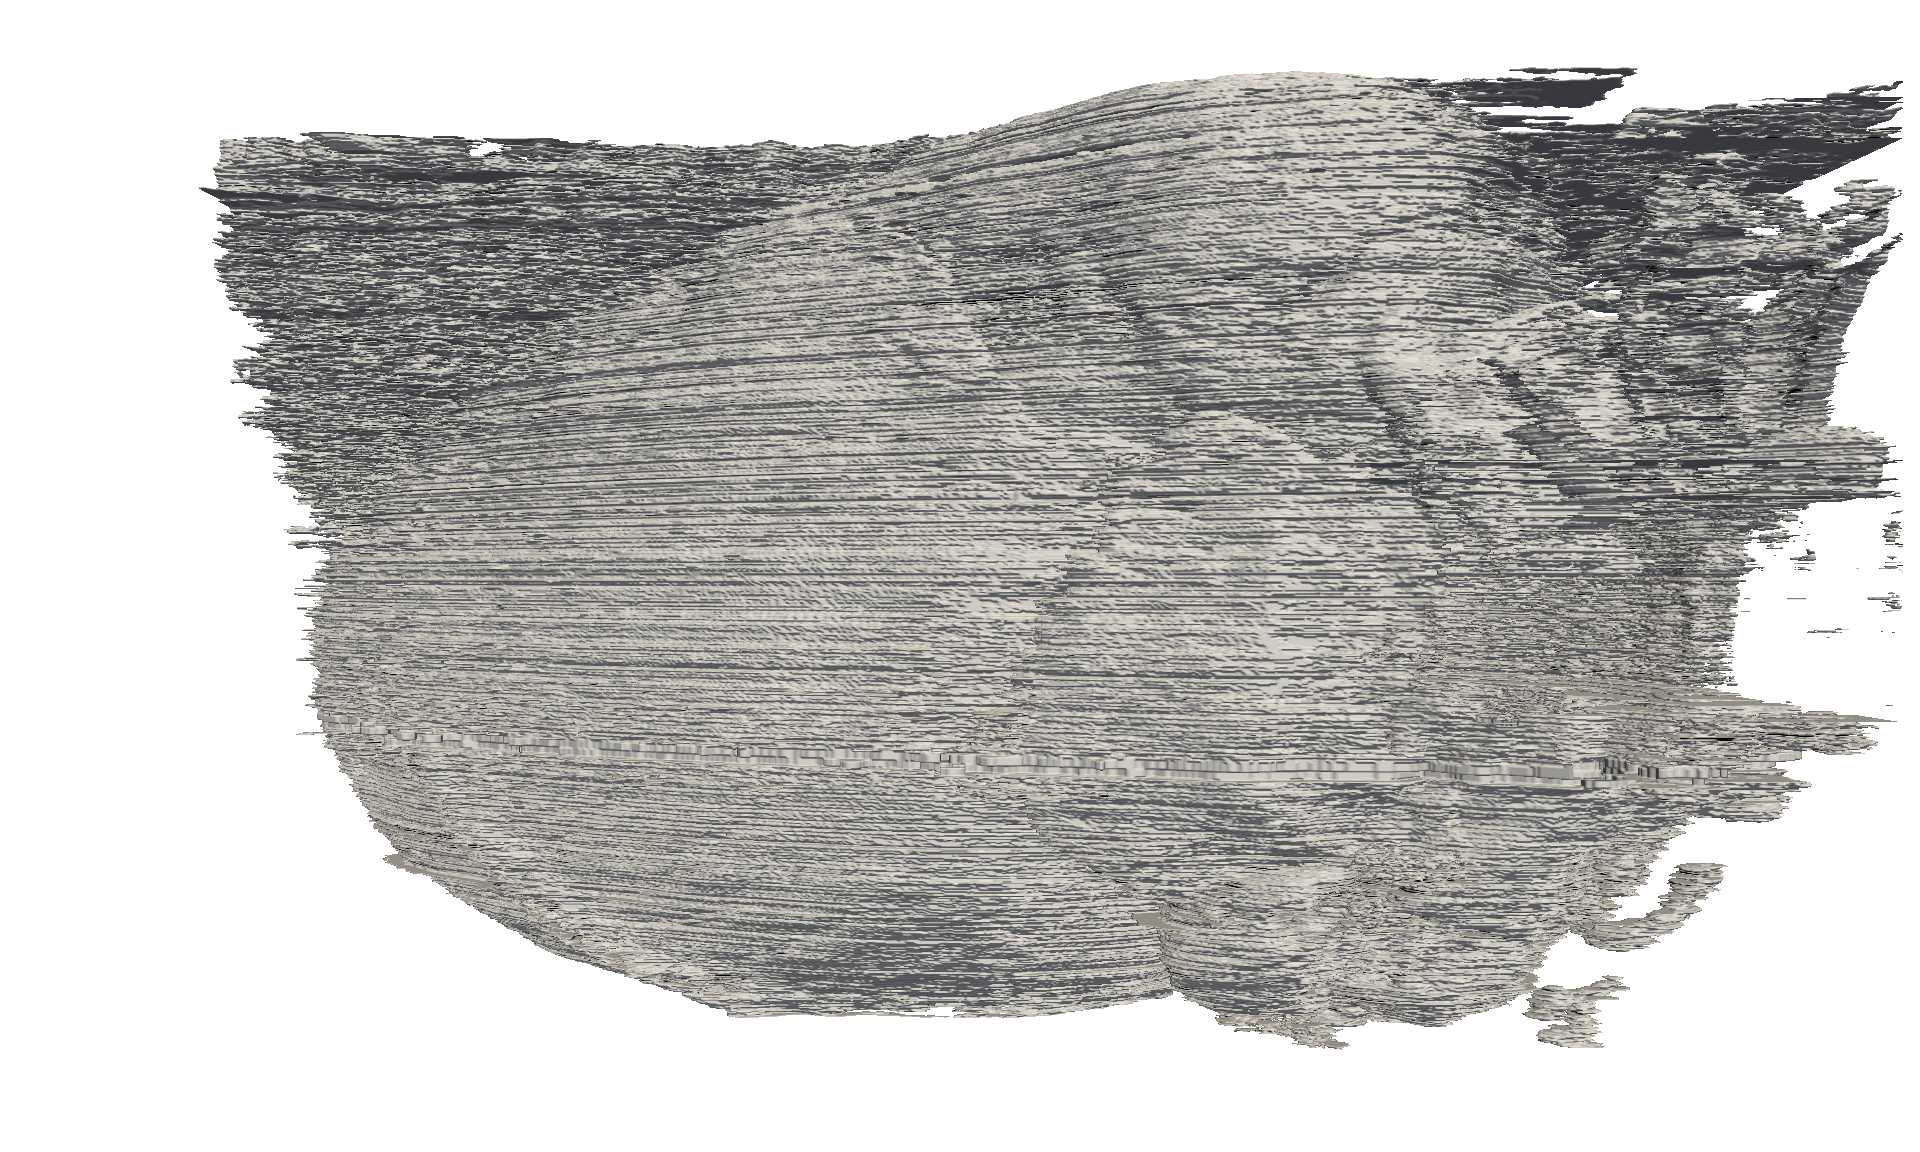
\includegraphics[width=\textheight]{Ch5/Figs/Rat28/contours/LoRes_negative_x}
    \caption{The block face contour viewed along the negative x direction. The more complex surface of the valve and vascular machinery at the base of the heart is visible to the right.}
    \label{fig:LoRes_negative_x}
  \end{sidewaysfigure}
    
  \begin{sidewaysfigure}[htbp]
    \centering
    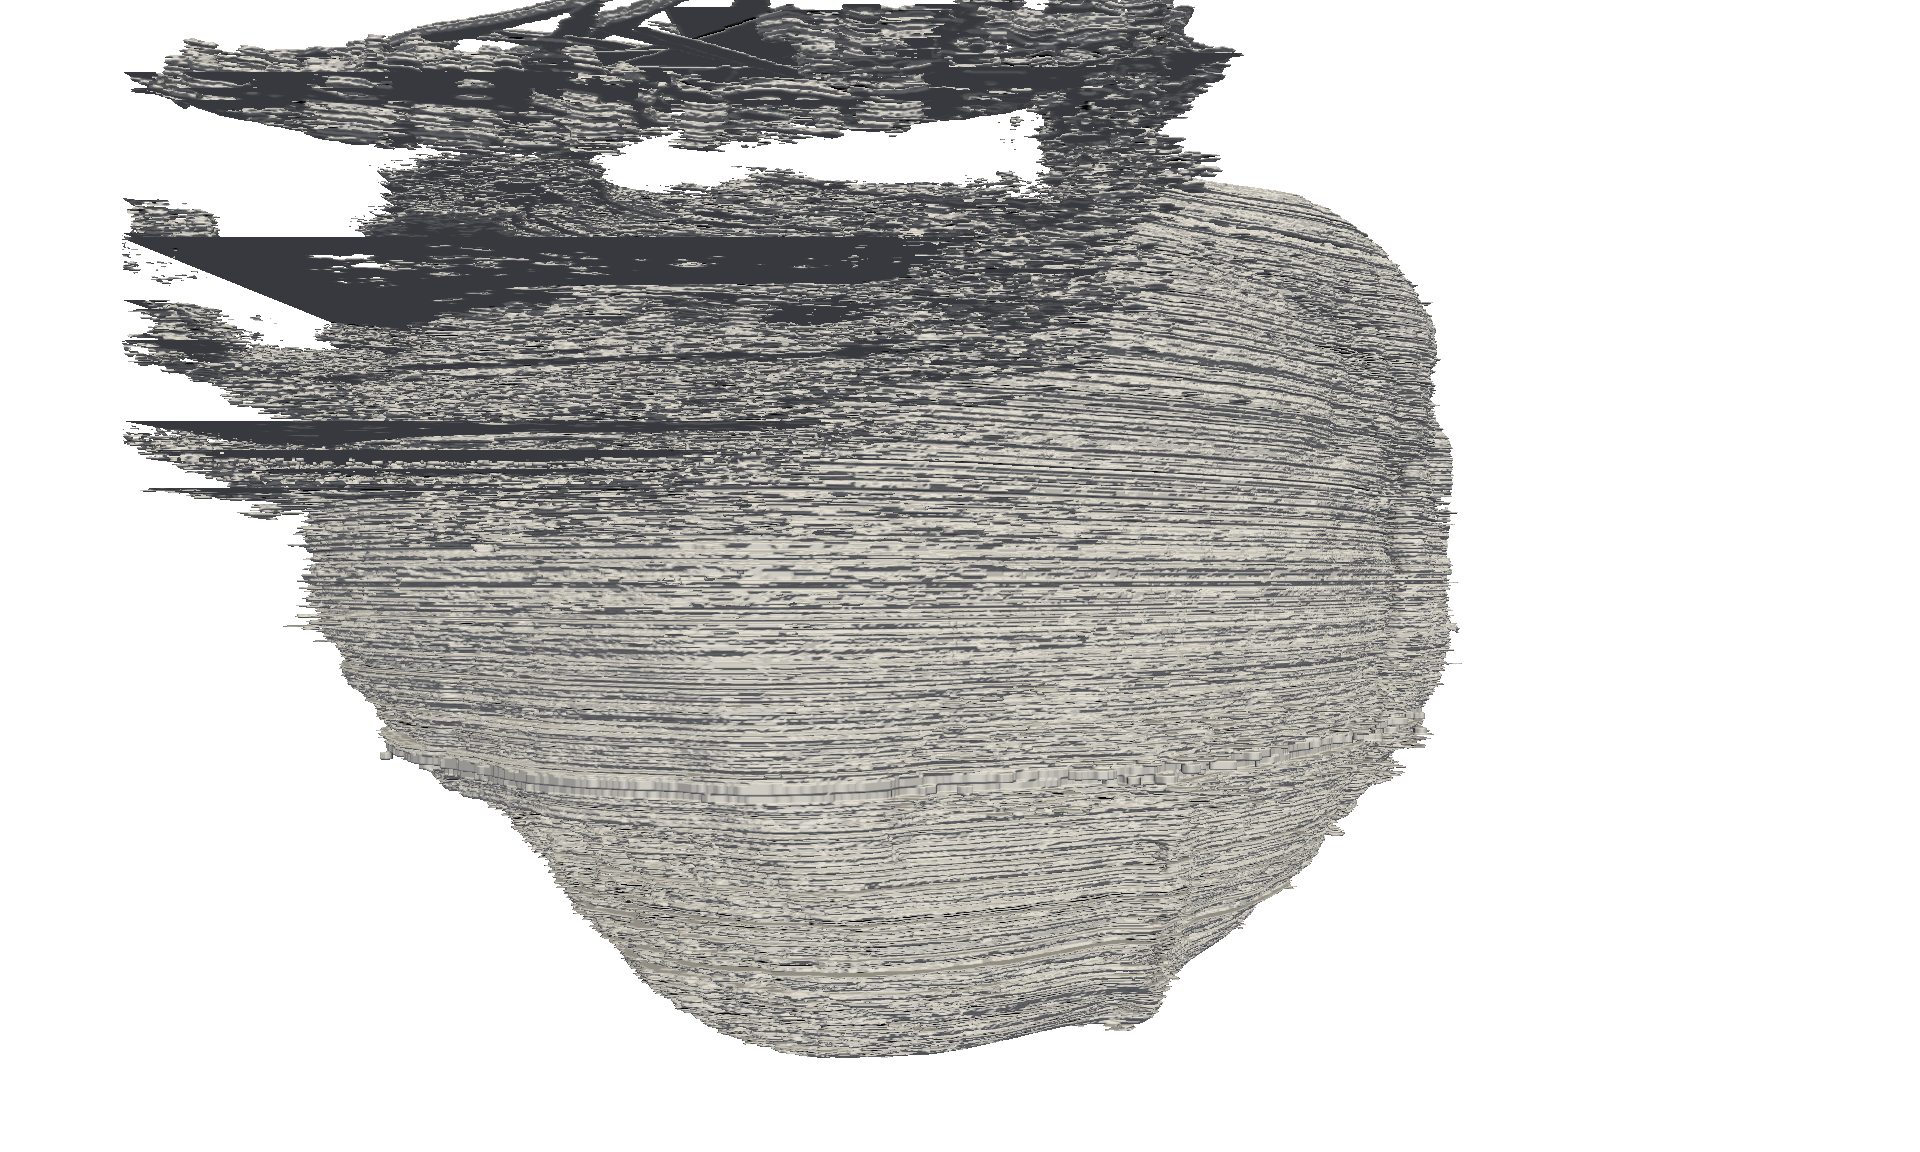
\includegraphics[width=\textheight]{Ch5/Figs/Rat28/contours/LoRes_positive_y}
    \caption{The block face contour viewed along the positive y direction. The bulge of an epicardial vessel at the bottom right hand side is clearly visible (it is also faintly visible towards the bottom left of Figure~\ref{fig:LoRes_negative_x}). The discrete change in illumination from Figure~\ref{subfig:LoRes_adjusted_long_cross_section} manifests as an apparent increase in surface size approximately a third of the height from the bottom.}
    \label{fig:LoRes_positive_y}
  \end{sidewaysfigure}
    
  \begin{sidewaysfigure}[htbp]
    \centering
    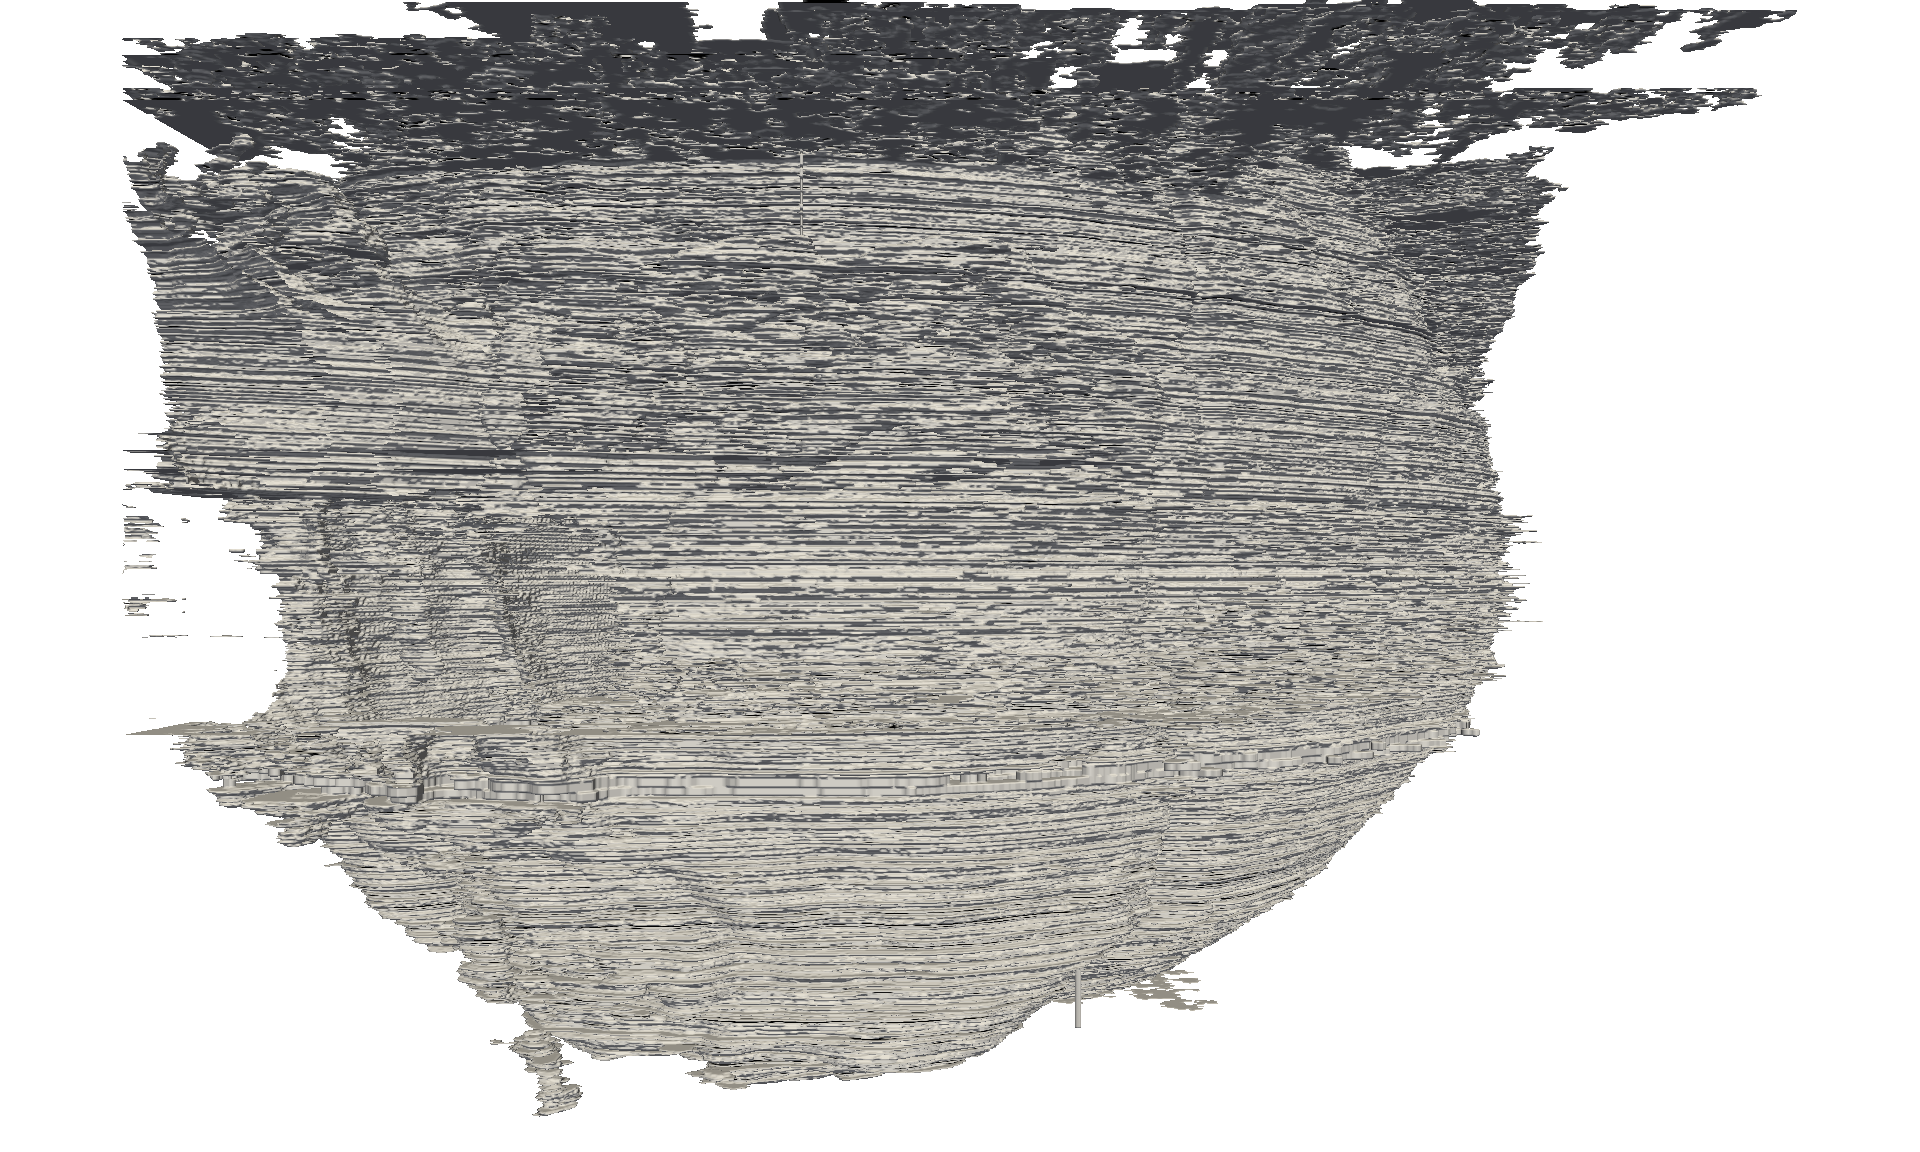
\includegraphics[width=\textheight]{Ch5/Figs/Rat28/contours/LoRes_negative_y}
    \caption{The block face contour viewed along the negative y direction.}
    \label{fig:LoRes_negative_y}
  \end{sidewaysfigure}
  
  \begin{sidewaysfigure}[htbp]
    \centering
    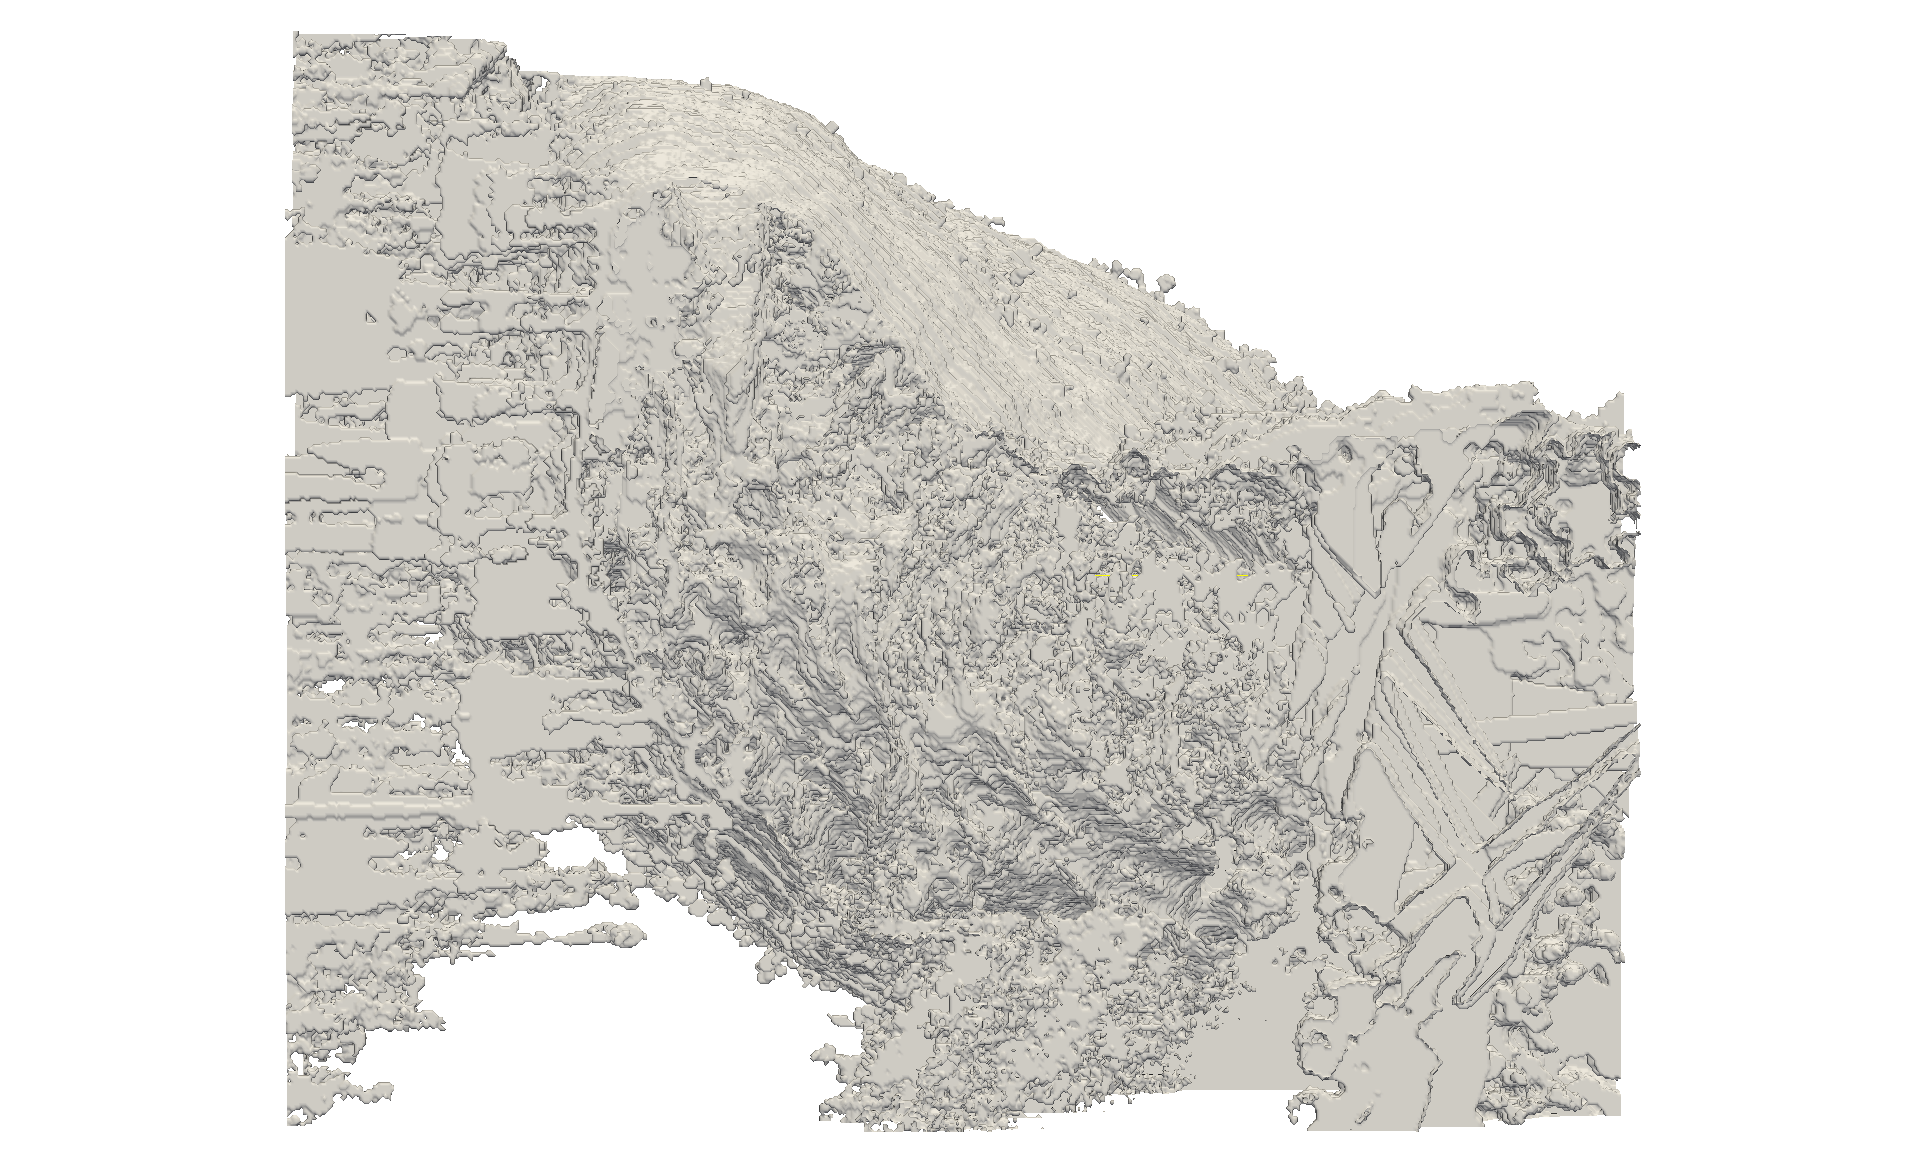
\includegraphics[width=\textheight]{Ch5/Figs/Rat28/contours/LoRes_negative_z}
    \caption{The block face contour viewed along the negative z direction. Bright reflection obscures much of the tissue surface from this angle, and the accurate registration of these top slices will prove impossible.}
    \label{fig:LoRes_negative_z}
  \end{sidewaysfigure}
  
	\begin{sidewaysfigure}[p]
	  \centering
	  
\includegraphics[width=0.9\textheight]{Ch6/Figs/Rat28/contours/whole_negative_x_geometric}
	  \caption{Geometrically initialised slice volume, viewed along the negative x direction.}
	  \label{fig:negative_x_geometric_contour}
	\end{sidewaysfigure}

	\begin{sidewaysfigure}[p]
	  \centering
	  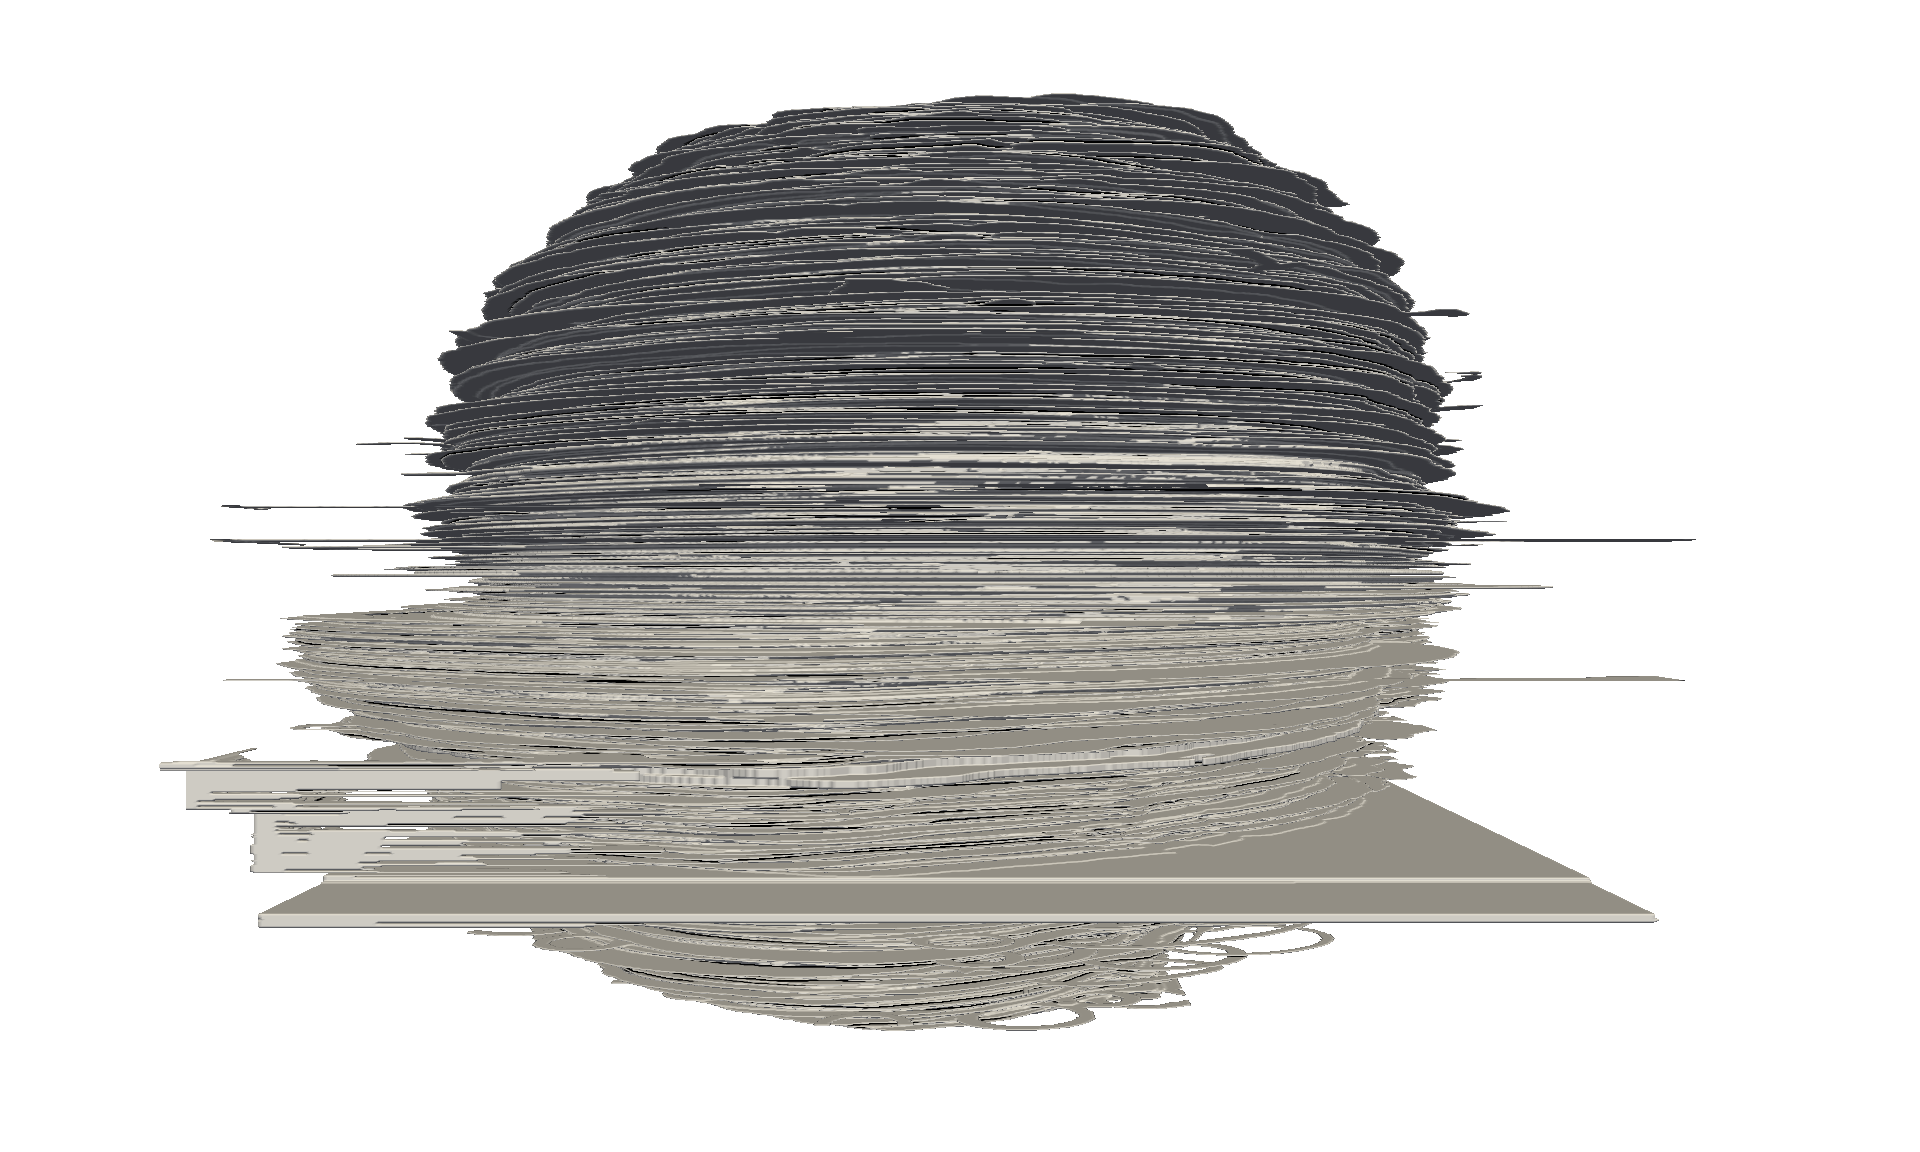
\includegraphics[width=0.9\textheight]{Ch6/Figs/Rat28/contours/whole_positive_y_geometric}
	  \caption{Geometrically initialised slice volume, viewed along the positive y direction.}
	  \label{fig:positive_y_geometric_contour}
	\end{sidewaysfigure}
  
	% rigid contours
	\begin{sidewaysfigure}[p]
	  \centering
	  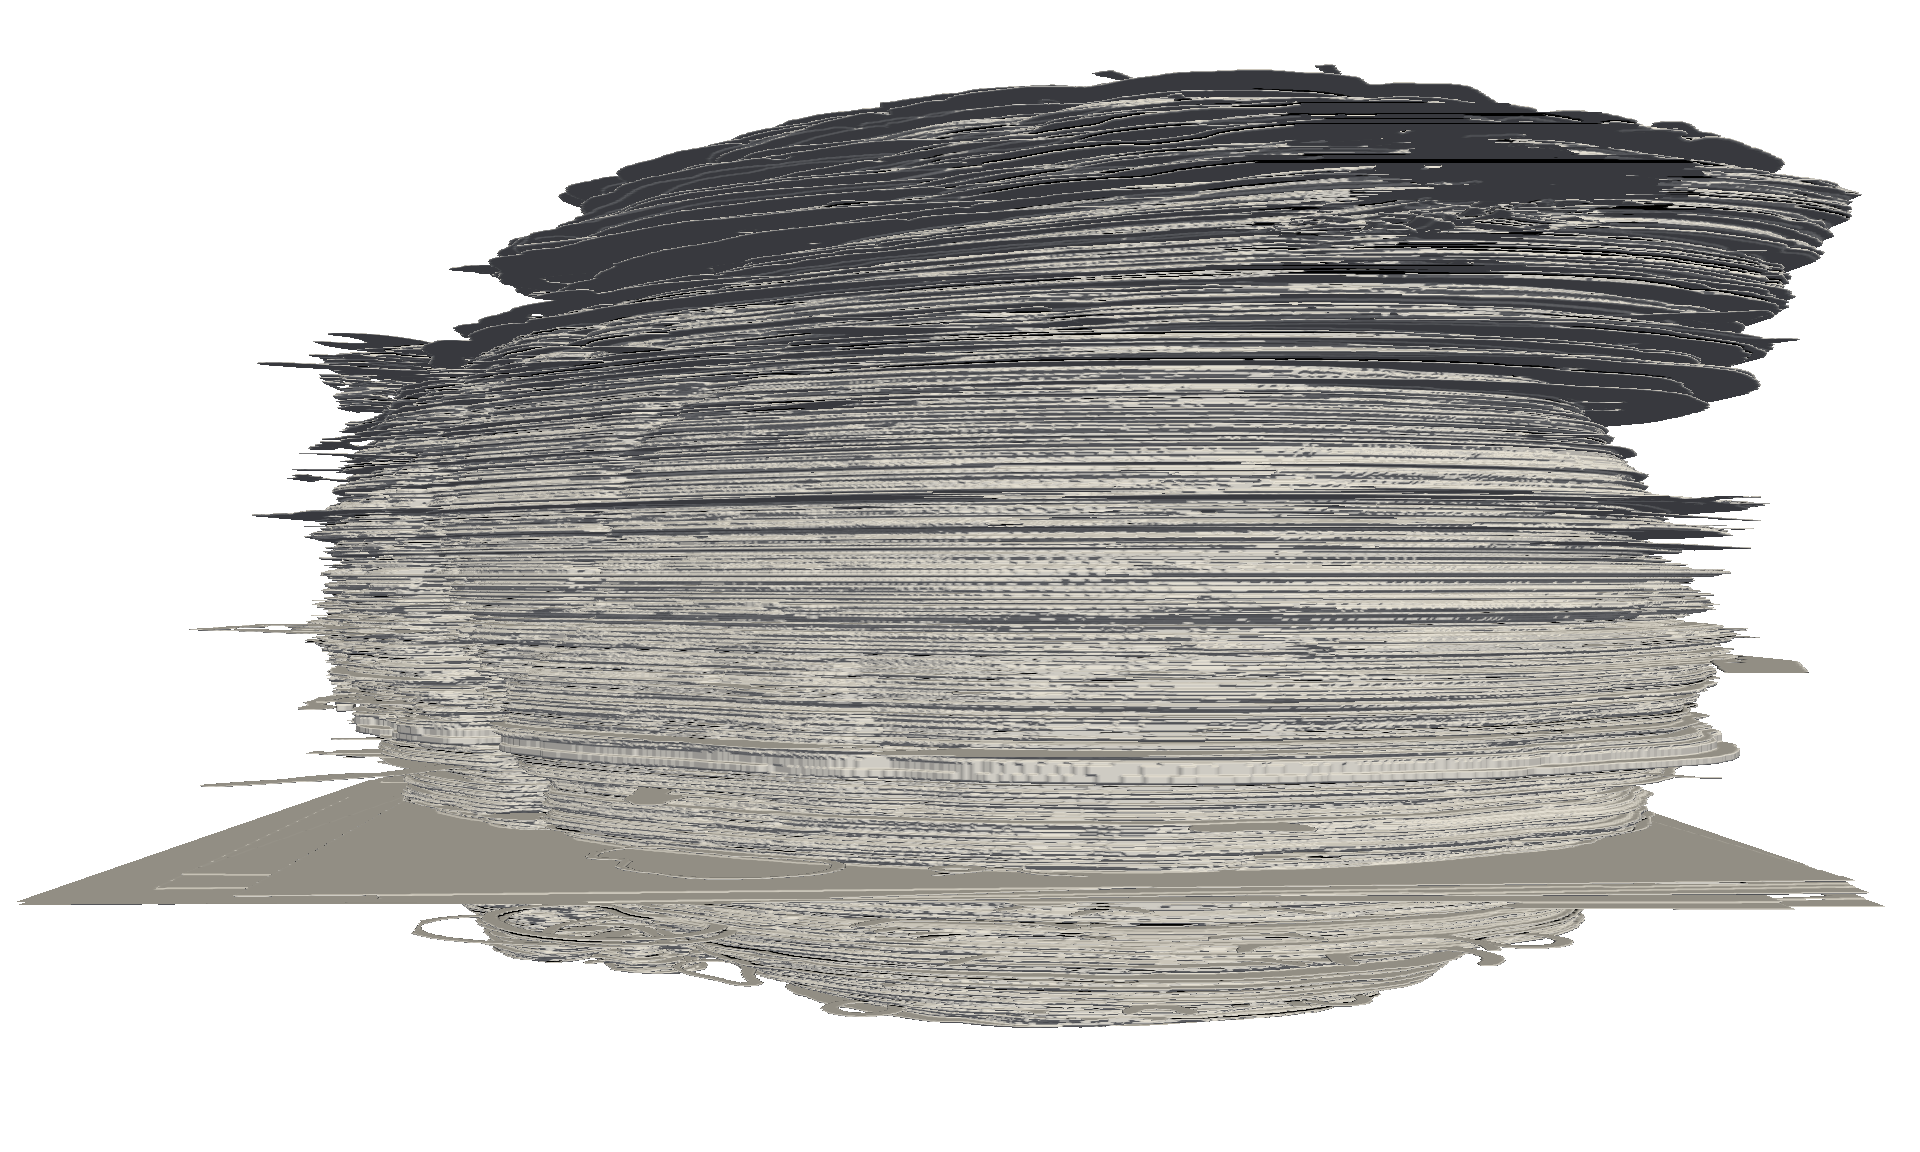
\includegraphics[width=0.9\textheight]{Ch6/Figs/Rat28/contours/whole_positive_x_rigid}
	  \caption{Rigid slice volume, viewed along the positive x direction.}
	  \label{fig:positive_x_rigid_contour}
	\end{sidewaysfigure}

	\begin{sidewaysfigure}[p]
	  \centering
	  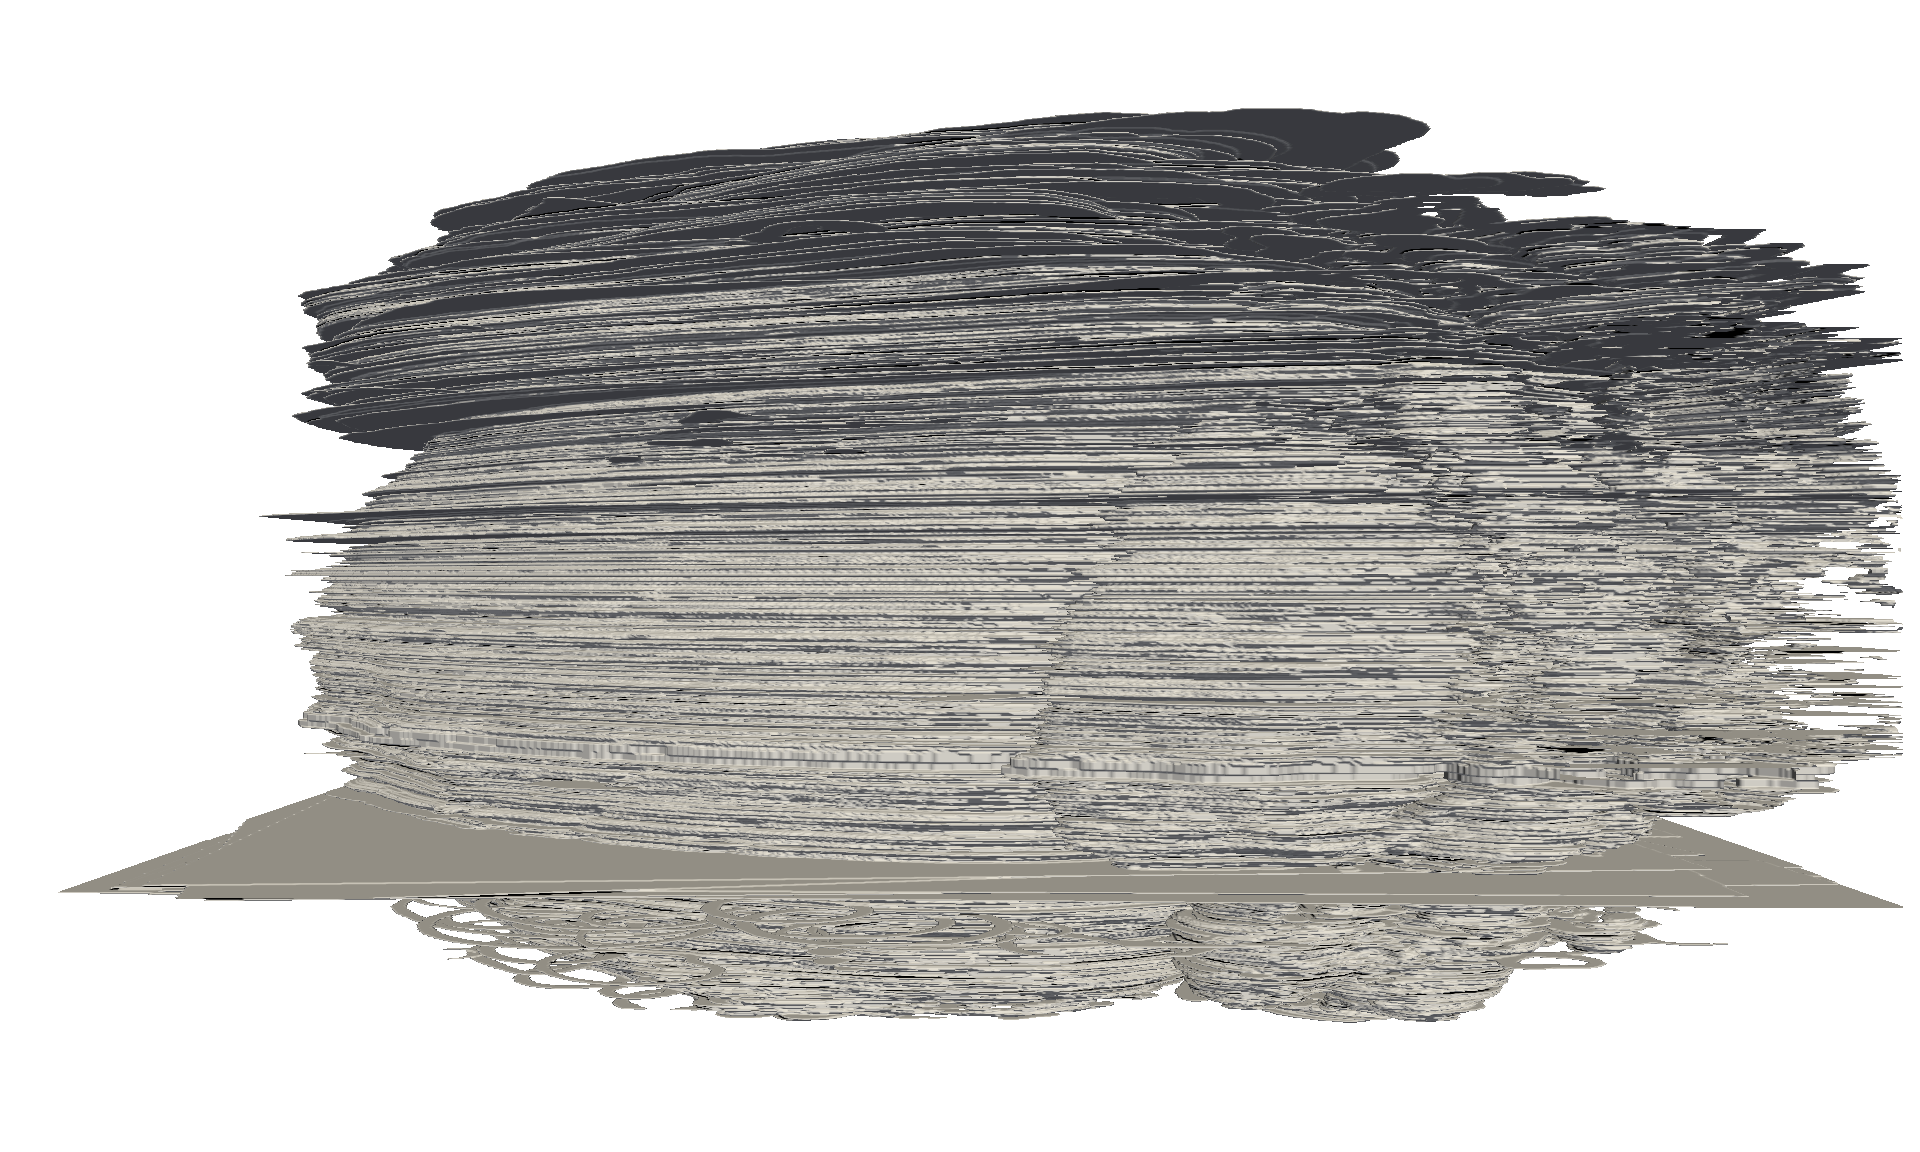
\includegraphics[width=0.9\textheight]{Ch6/Figs/Rat28/contours/whole_negative_x_rigid}
	  \caption{Rigid slice volume, viewed along the negative x direction.}
	  \label{fig:negative_x_rigid_contour}
	\end{sidewaysfigure}

	\begin{sidewaysfigure}[p]
	  \centering
	  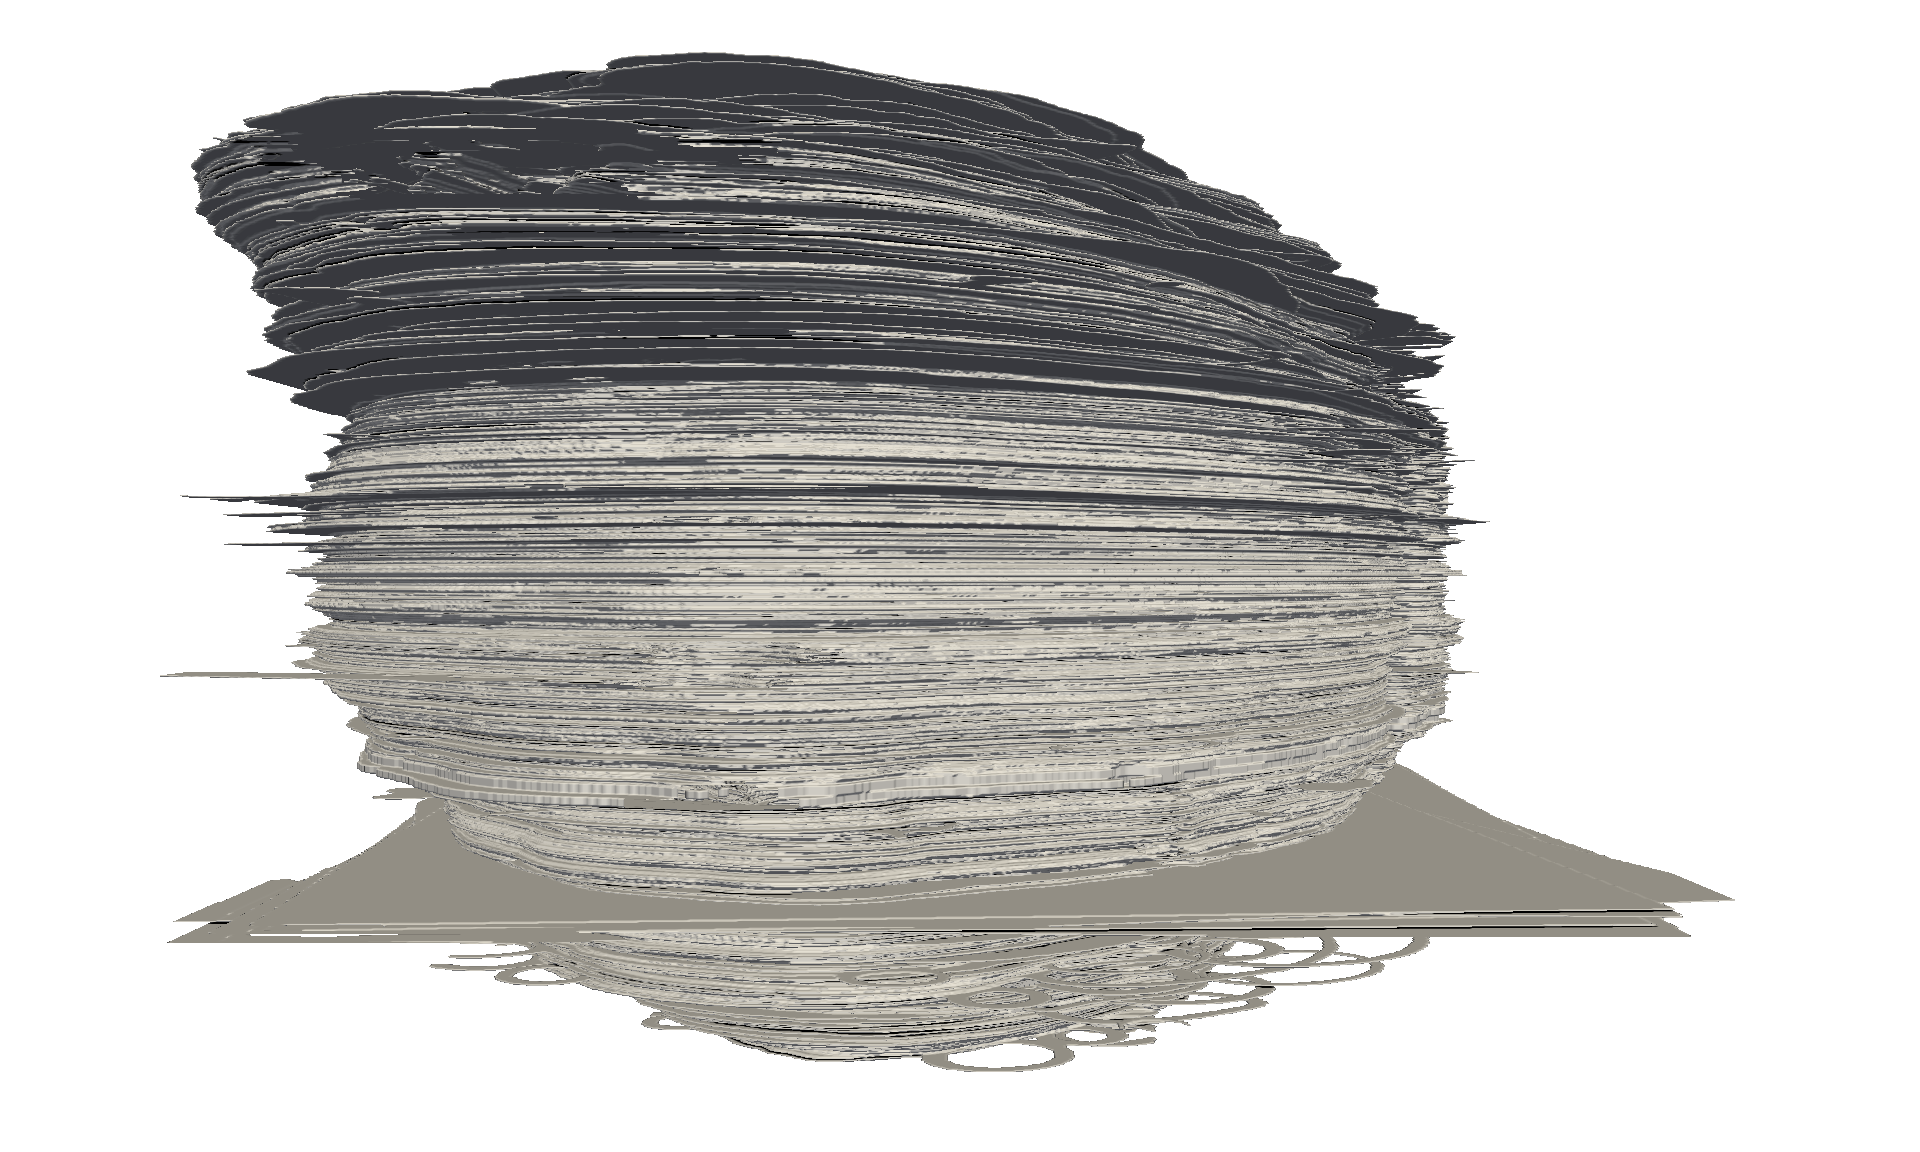
\includegraphics[width=0.9\textheight]{Ch6/Figs/Rat28/contours/whole_positive_y_rigid}
	  \caption{Rigid slice volume, viewed along the positive y direction.}
	  \label{fig:positive_y_rigid_contour}
	\end{sidewaysfigure}

	\begin{sidewaysfigure}[p]
	  \centering
	  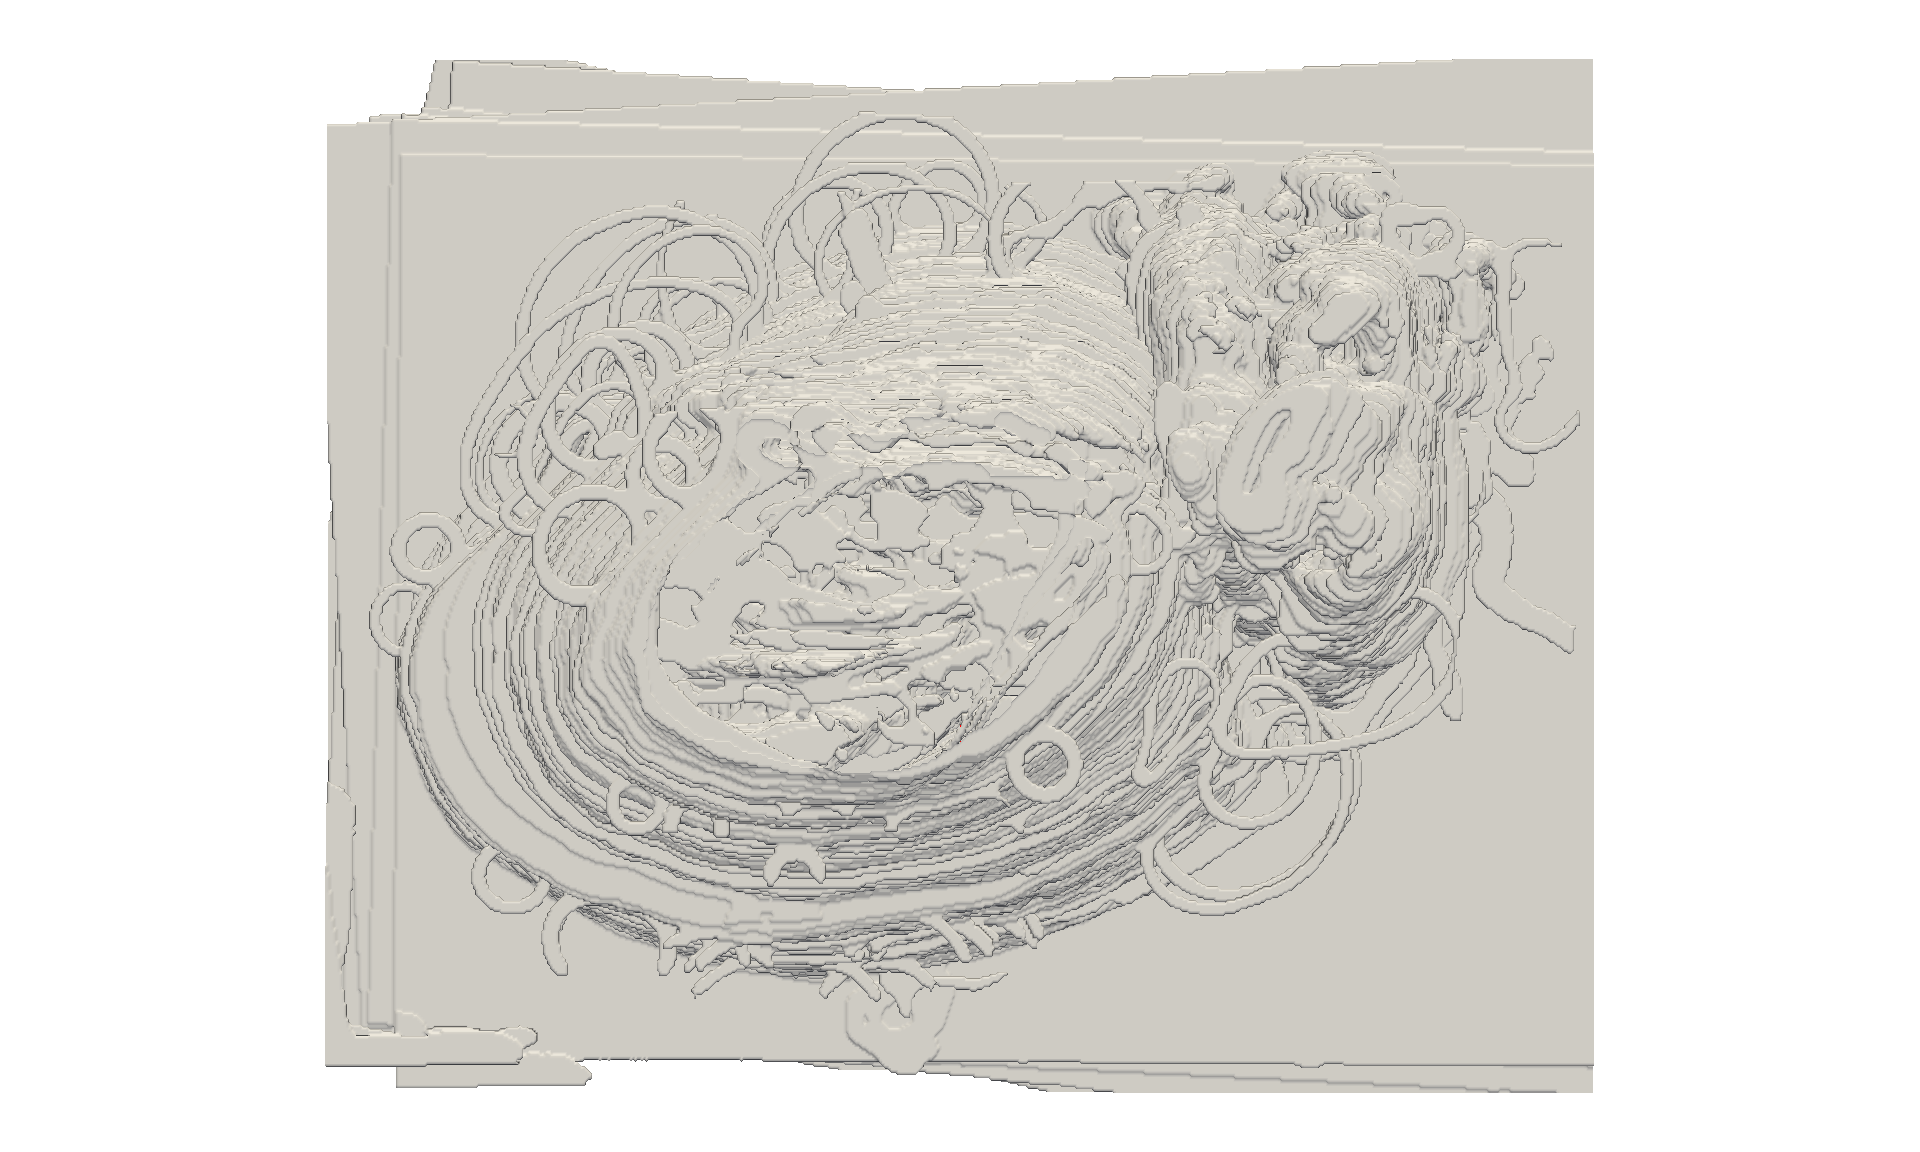
\includegraphics[width=0.9\textheight]{Ch6/Figs/Rat28/contours/whole_positive_z_rigid}
	  \caption{Rigid slice volume, viewed along the positive z direction.}
	  \label{fig:positive_z_rigid_contour}
	\end{sidewaysfigure}

	% size contours
	\begin{sidewaysfigure}[p]
	  \centering
	  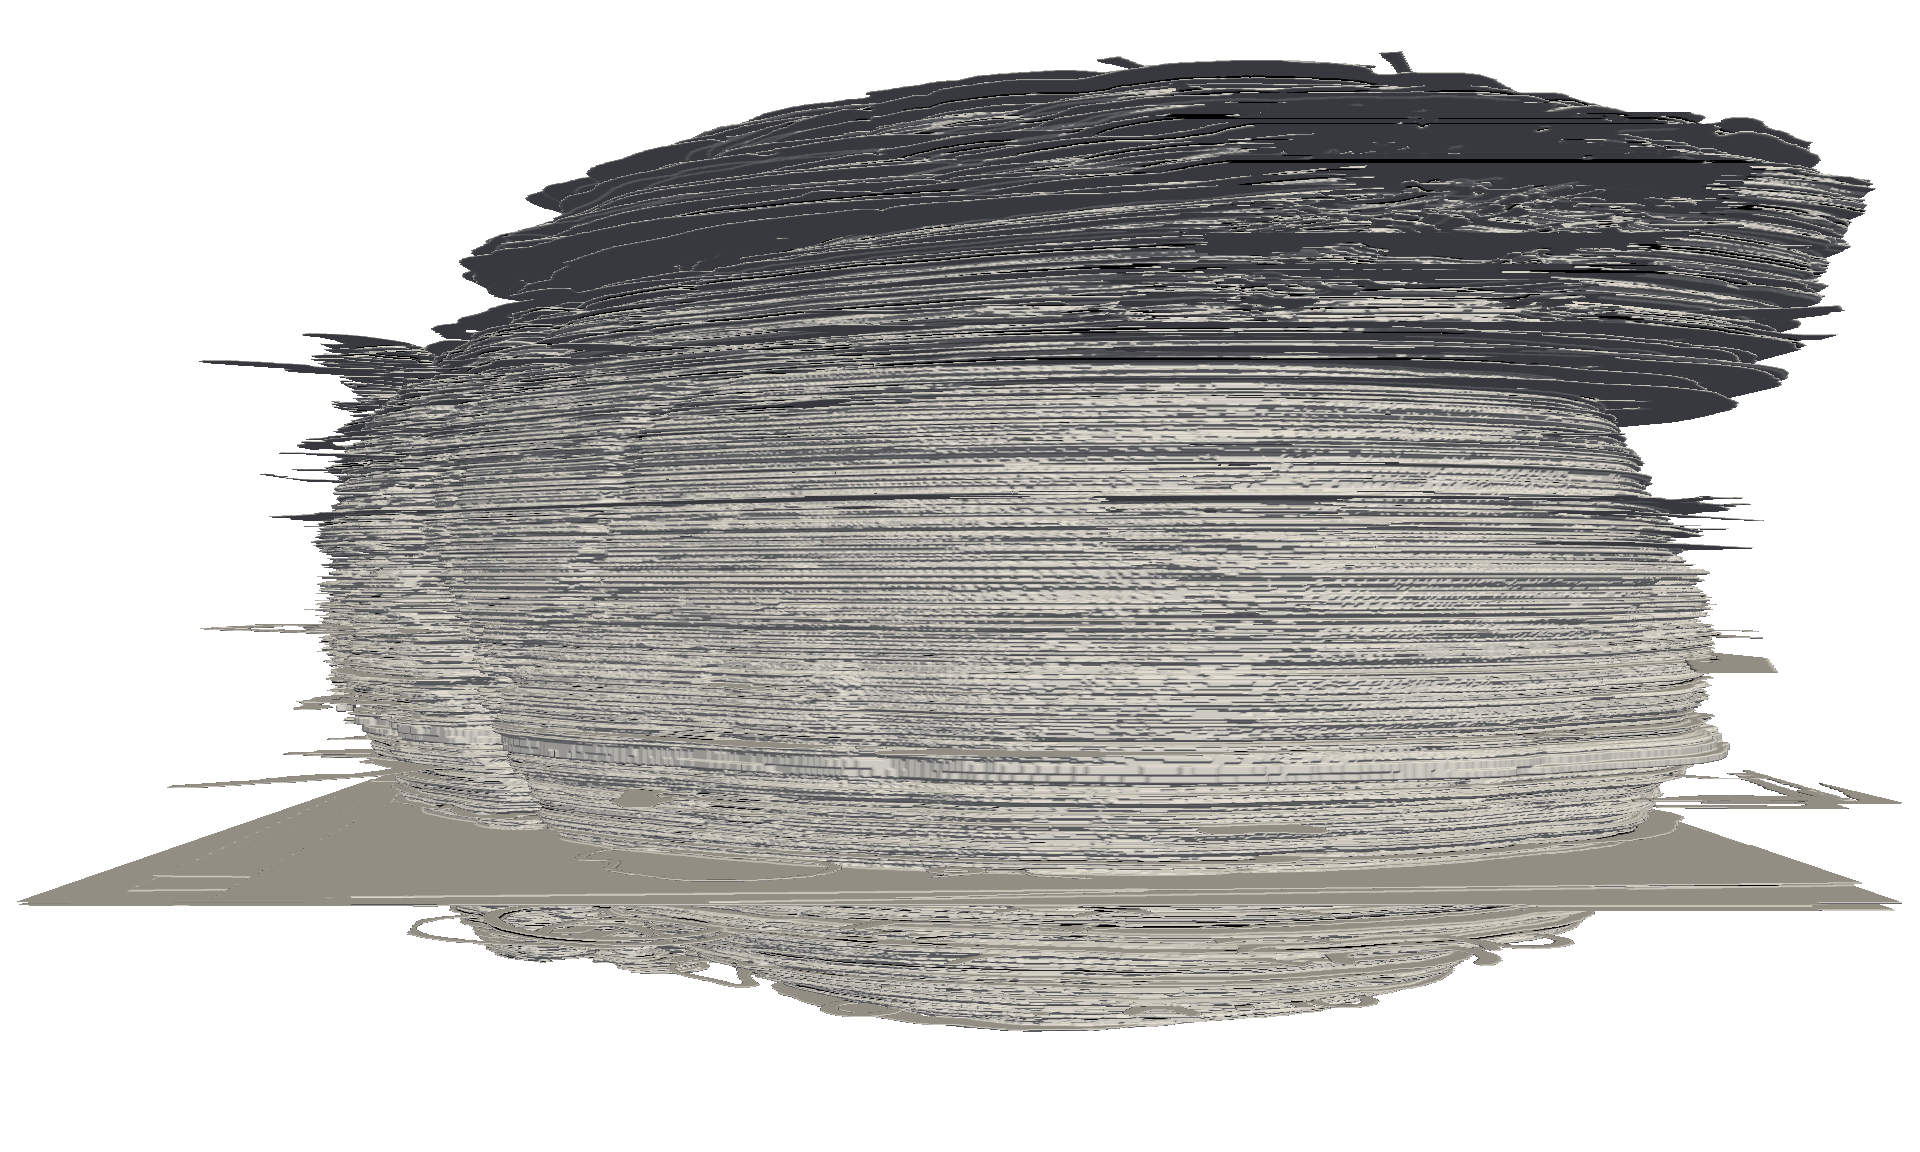
\includegraphics[width=0.9\textheight]{Ch6/Figs/Rat28/contours/whole_positive_x_size}
	  \caption{Similarity slice volume, viewed along the positive x direction.}
	  \label{fig:positive_x_similarity_contour}
	\end{sidewaysfigure}

	\begin{sidewaysfigure}[p]
	  \centering
	  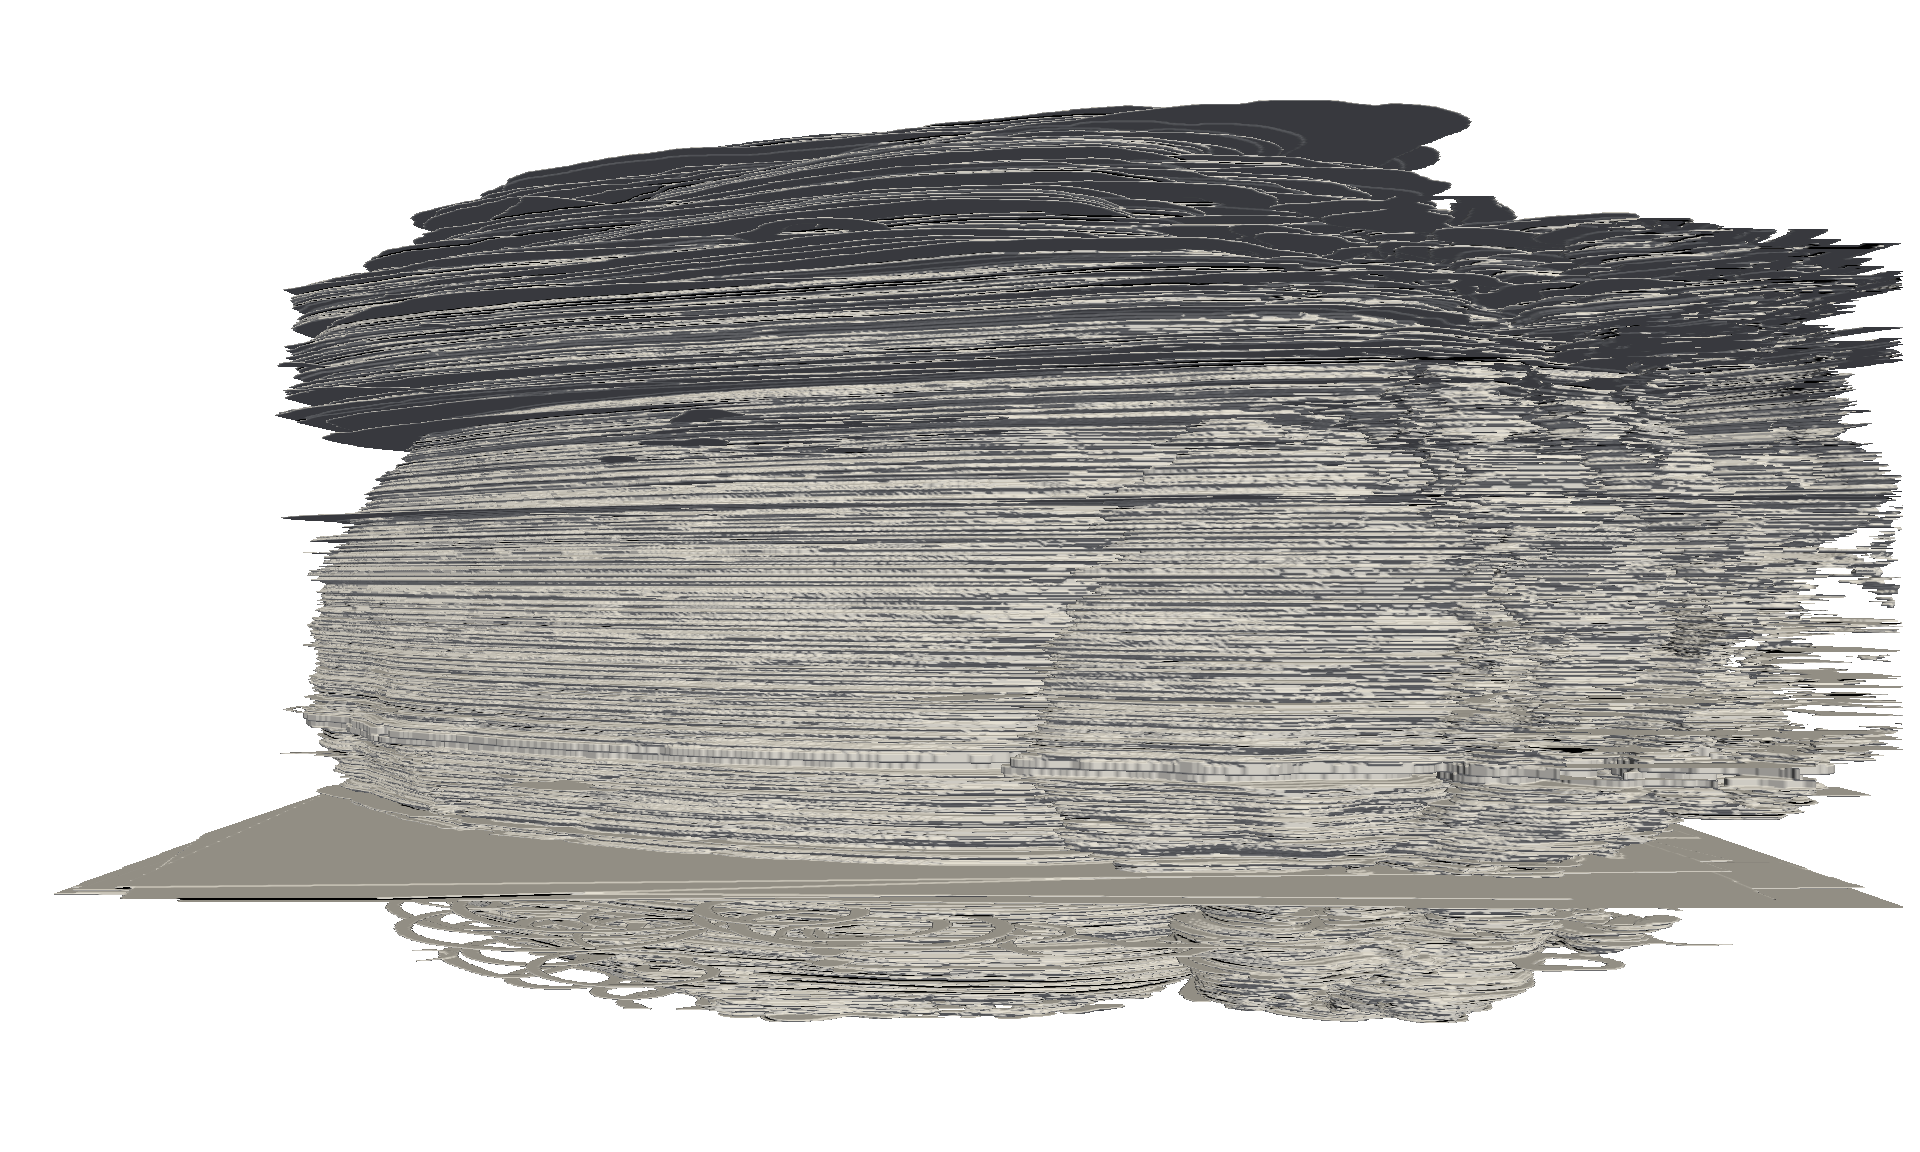
\includegraphics[width=0.9\textheight]{Ch6/Figs/Rat28/contours/whole_negative_x_size}
	  \caption{Similarity slice volume, viewed along the negative x direction.}
	  \label{fig:negative_x_similarity_contour}
	\end{sidewaysfigure}

	\begin{sidewaysfigure}[p]
	  \centering
	  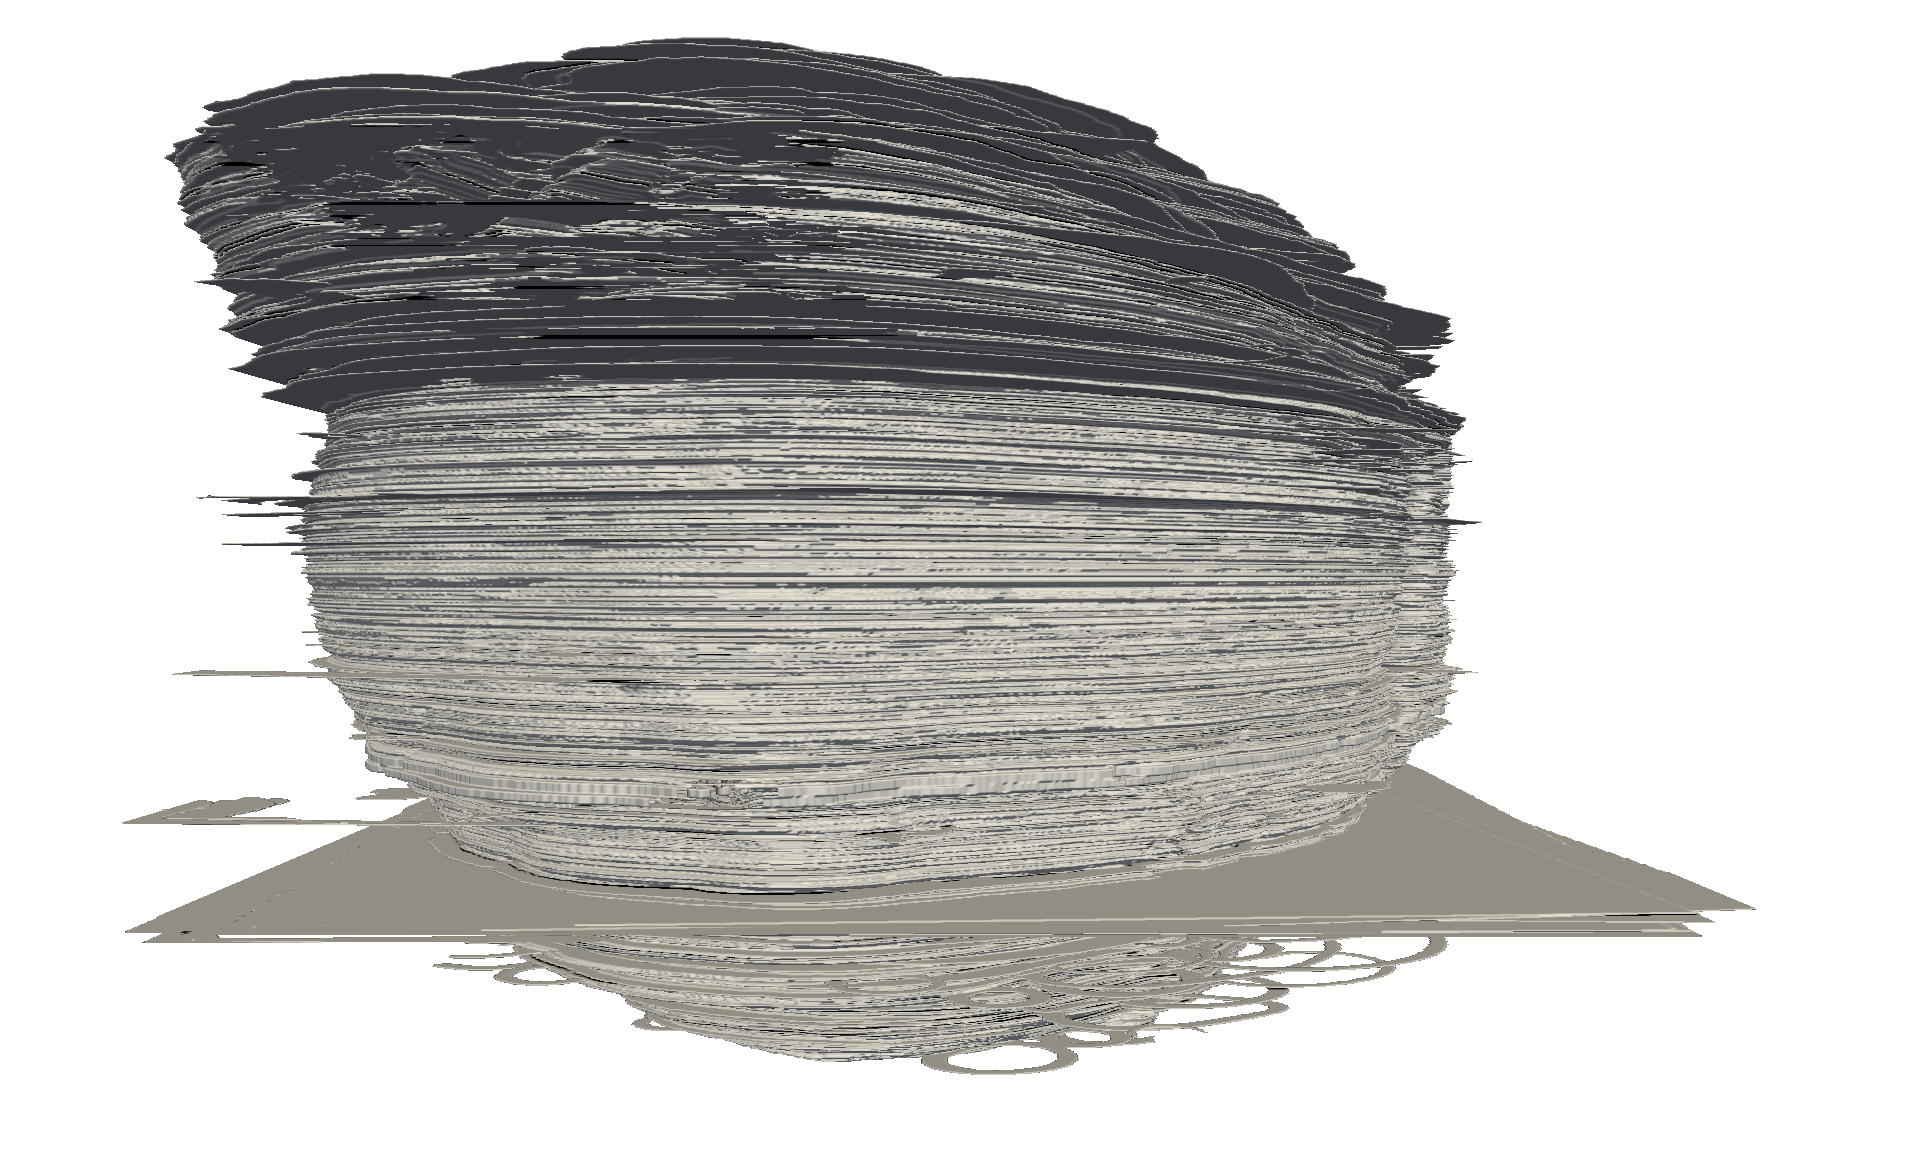
\includegraphics[width=0.9\textheight]{Ch6/Figs/Rat28/contours/whole_positive_y_size}
	  \caption{Similarity slice volume, viewed along the positive y direction.}
	  \label{fig:positive_y_similarity_contour}
	\end{sidewaysfigure}

	\begin{sidewaysfigure}[p]
	  \centering
	  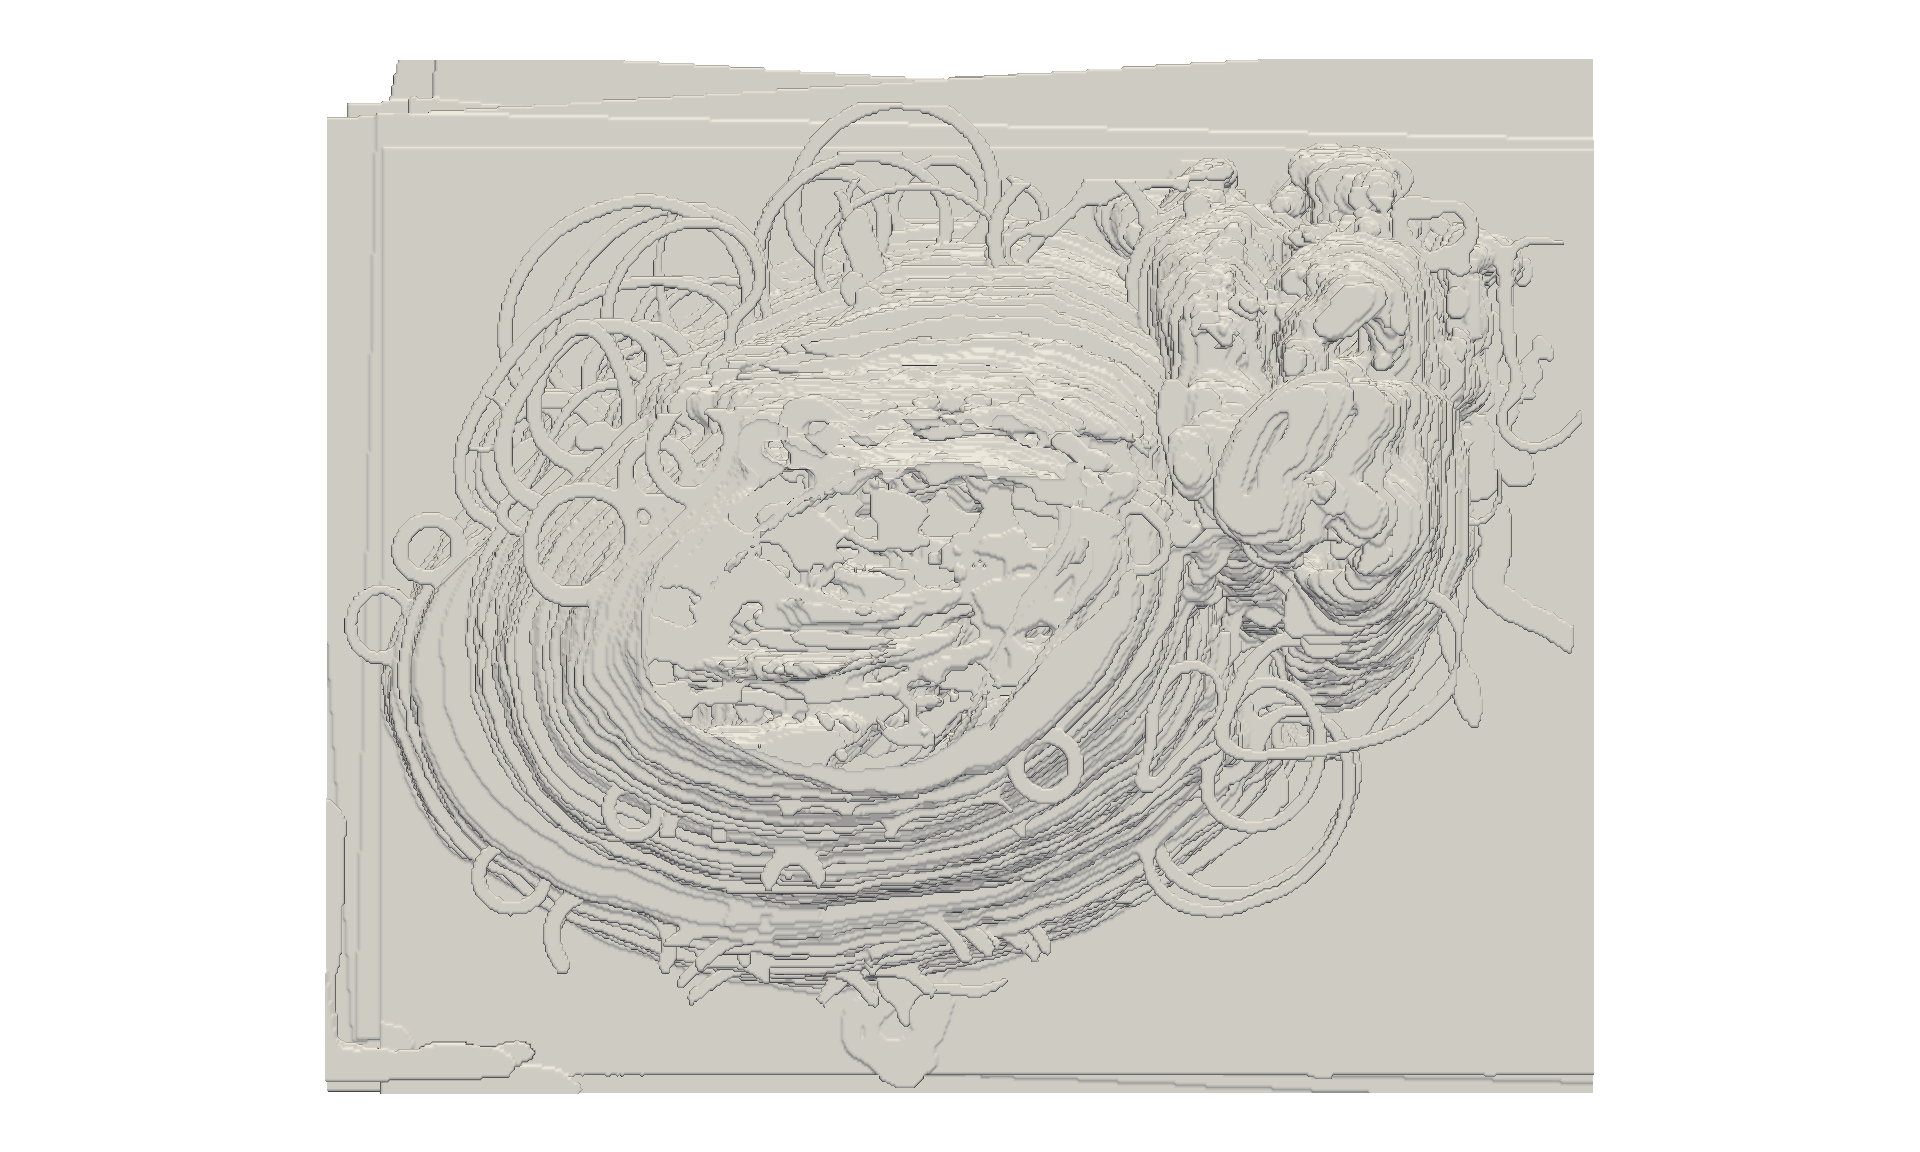
\includegraphics[width=0.9\textheight]{Ch6/Figs/Rat28/contours/whole_positive_z_size}
	  \caption{Similarity slice volume, viewed along the positive z direction.}
	  \label{fig:positive_z_similarity_contour}
	\end{sidewaysfigure}

	\begin{sidewaysfigure}[p]
	  \centering
	  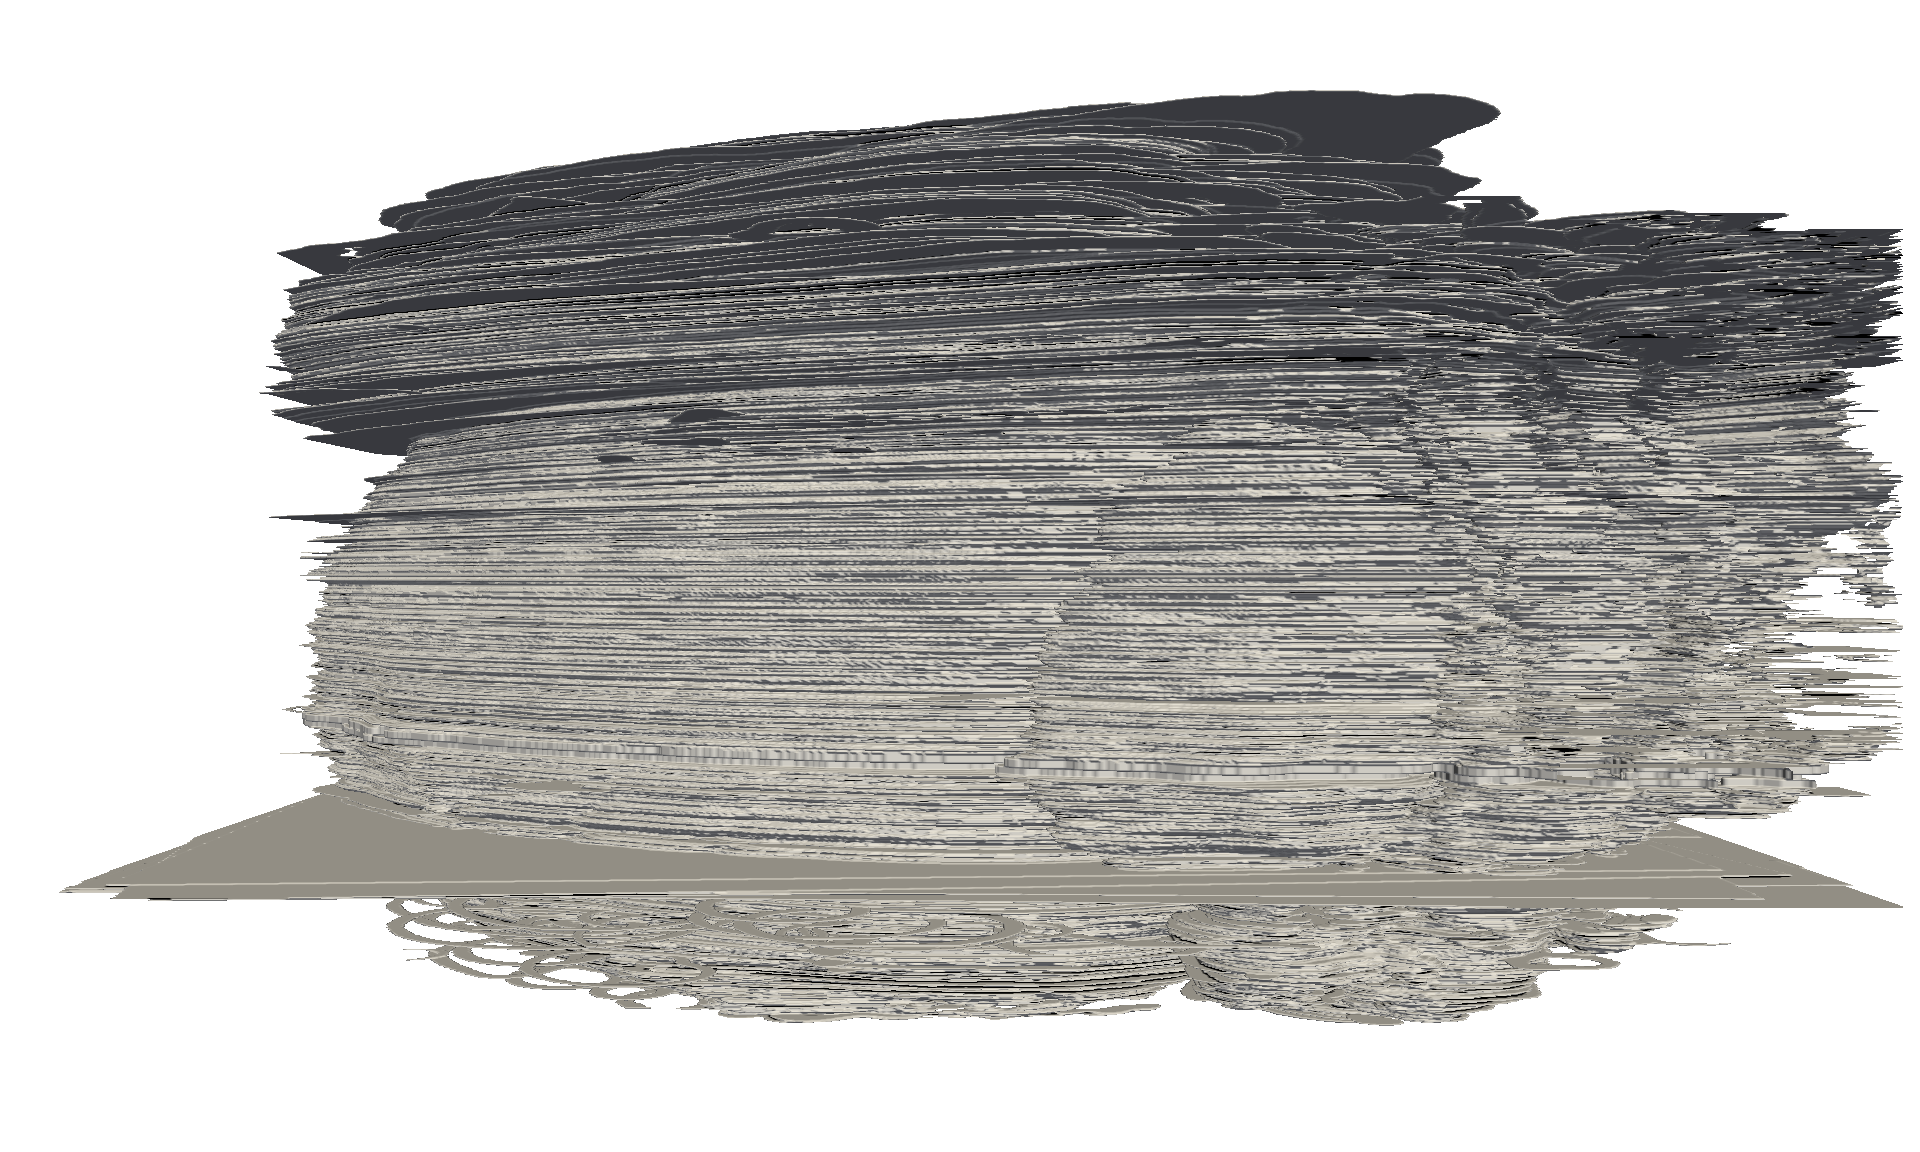
\includegraphics[width=0.9\textheight]{Ch6/Figs/Rat28/contours/whole_negative_x_affine}
	  \caption{Affine slice volume, viewed along the negative x direction.}
	  \label{fig:negative_x_affine_contour}
	\end{sidewaysfigure}

	\begin{sidewaysfigure}[p]
	  \centering
	  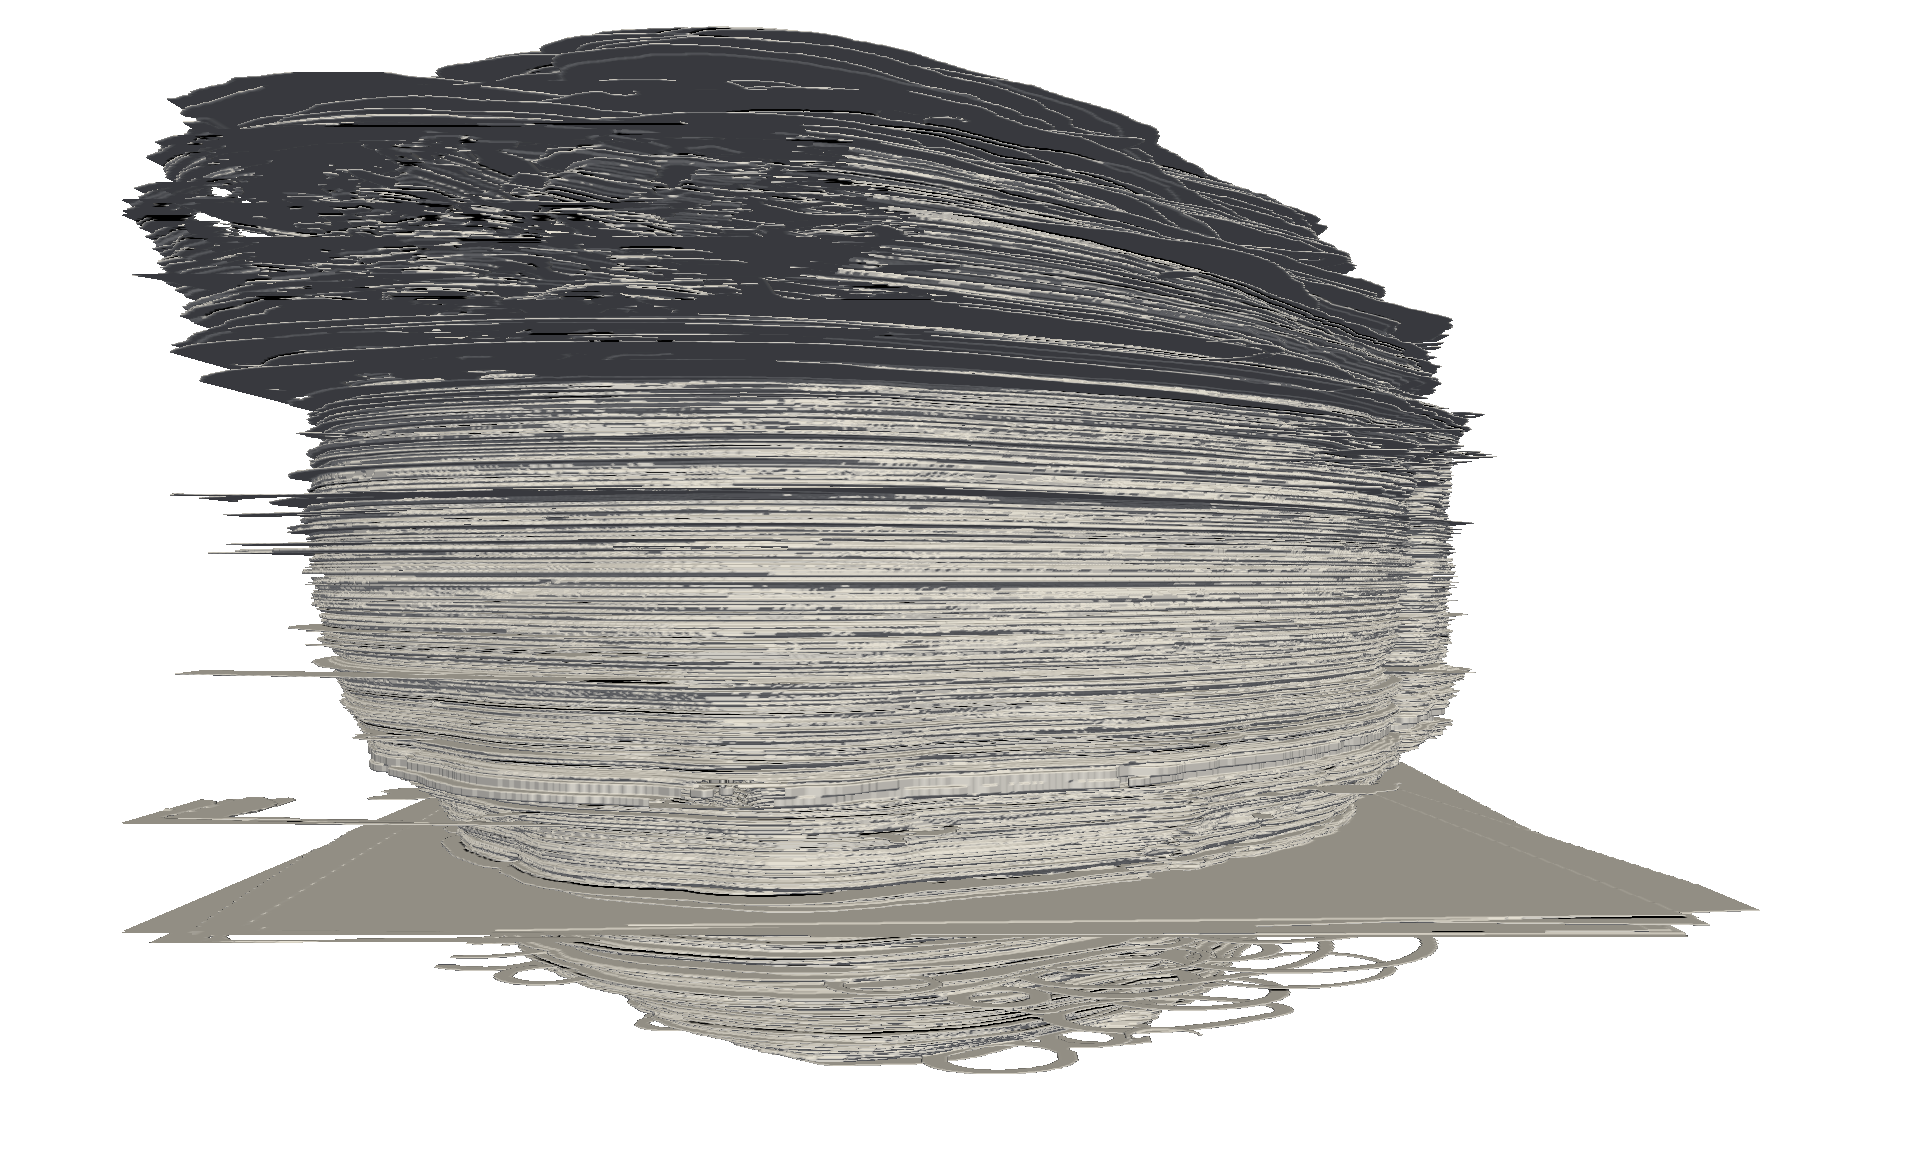
\includegraphics[width=0.9\textheight]{Ch6/Figs/Rat28/contours/whole_positive_y_affine}
	  \caption{Affine slice volume, viewed along the positive y direction.}
	  \label{fig:positive_y_affine_contour}
	\end{sidewaysfigure}

  \begin{sidewaysfigure}[p]
    \centering
    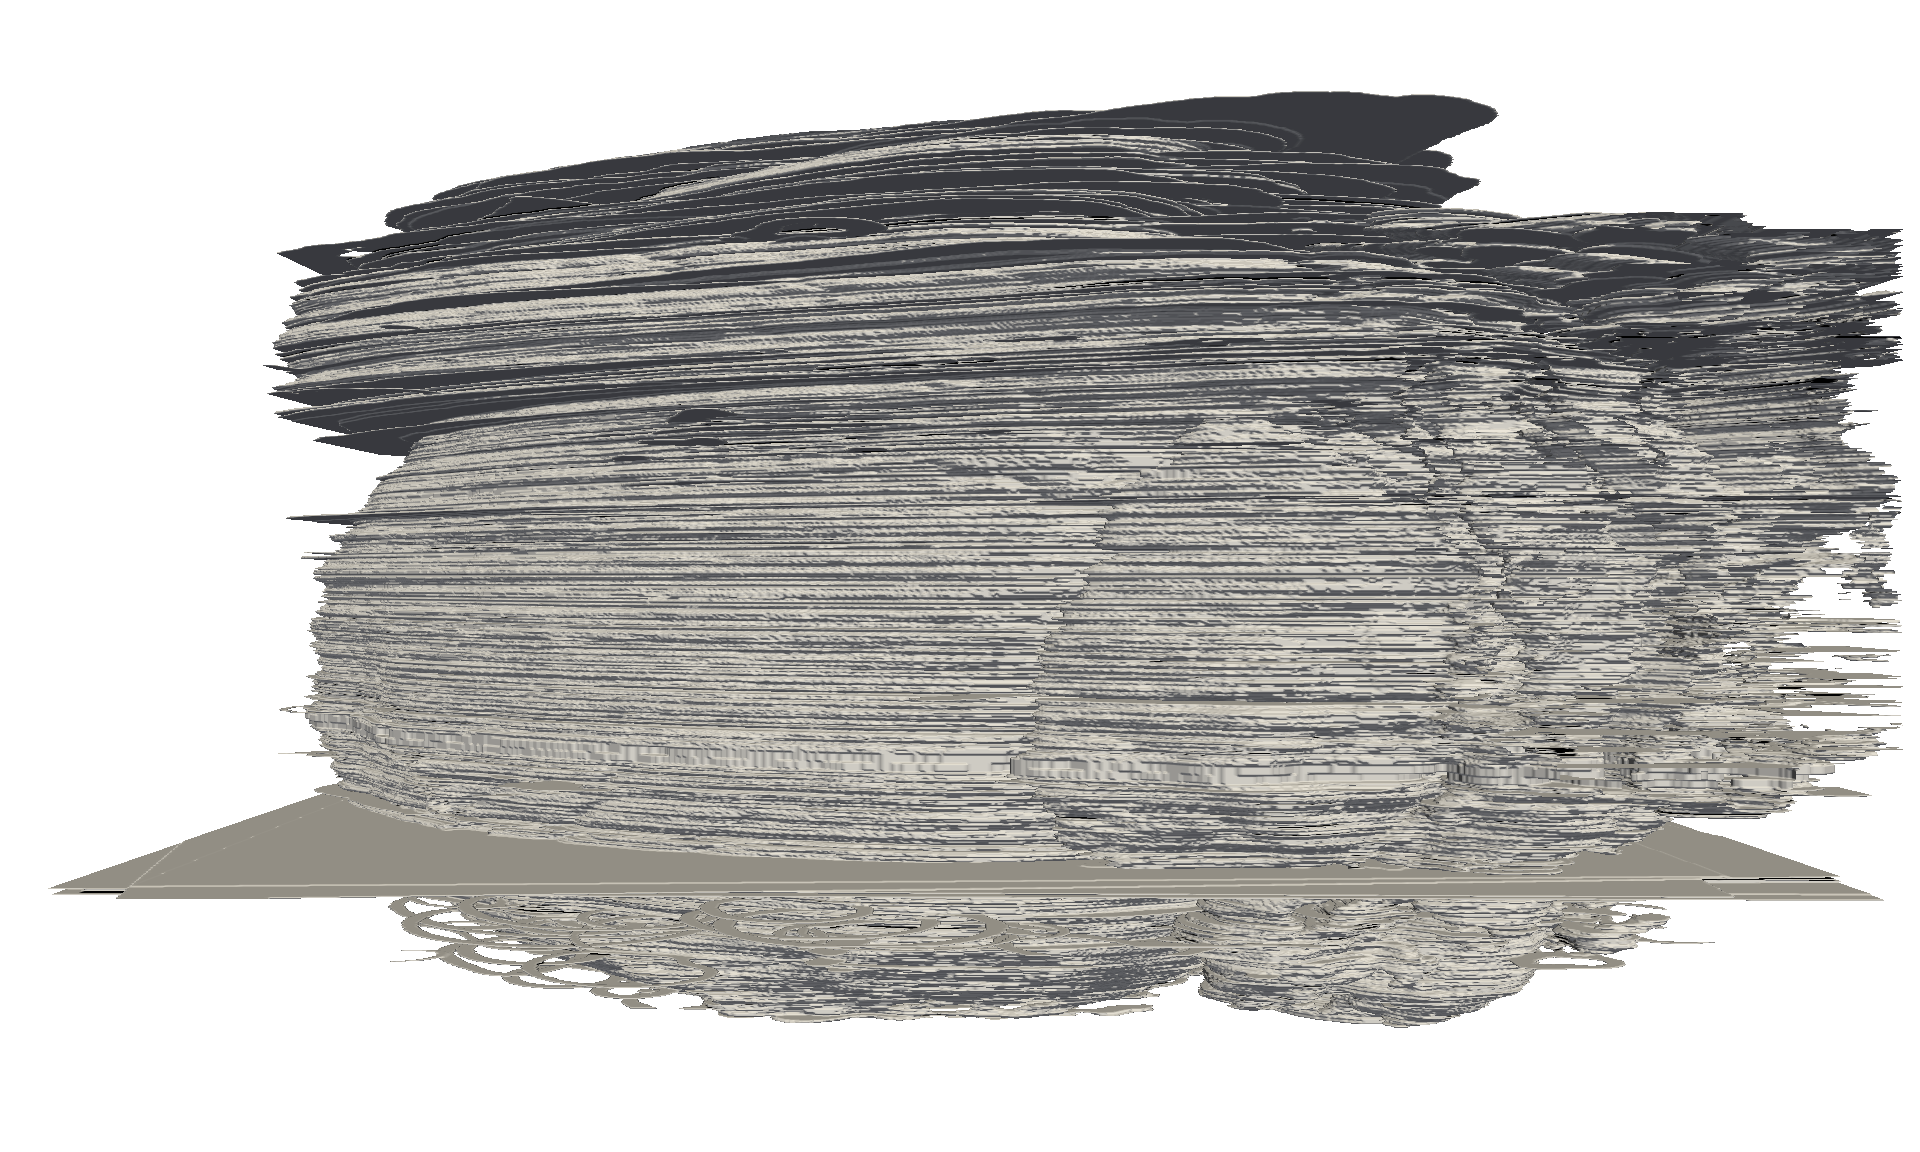
\includegraphics[width=0.9\textheight]{Ch6/Figs/Rat28/contours/whole_negative_x_diffused}
    \caption{Globally smoothed slice volume, viewed along the negative x direction.}
    \label{fig:whole_negative_x_diffused}
  \end{sidewaysfigure}

  \begin{sidewaysfigure}[p]
    \centering
    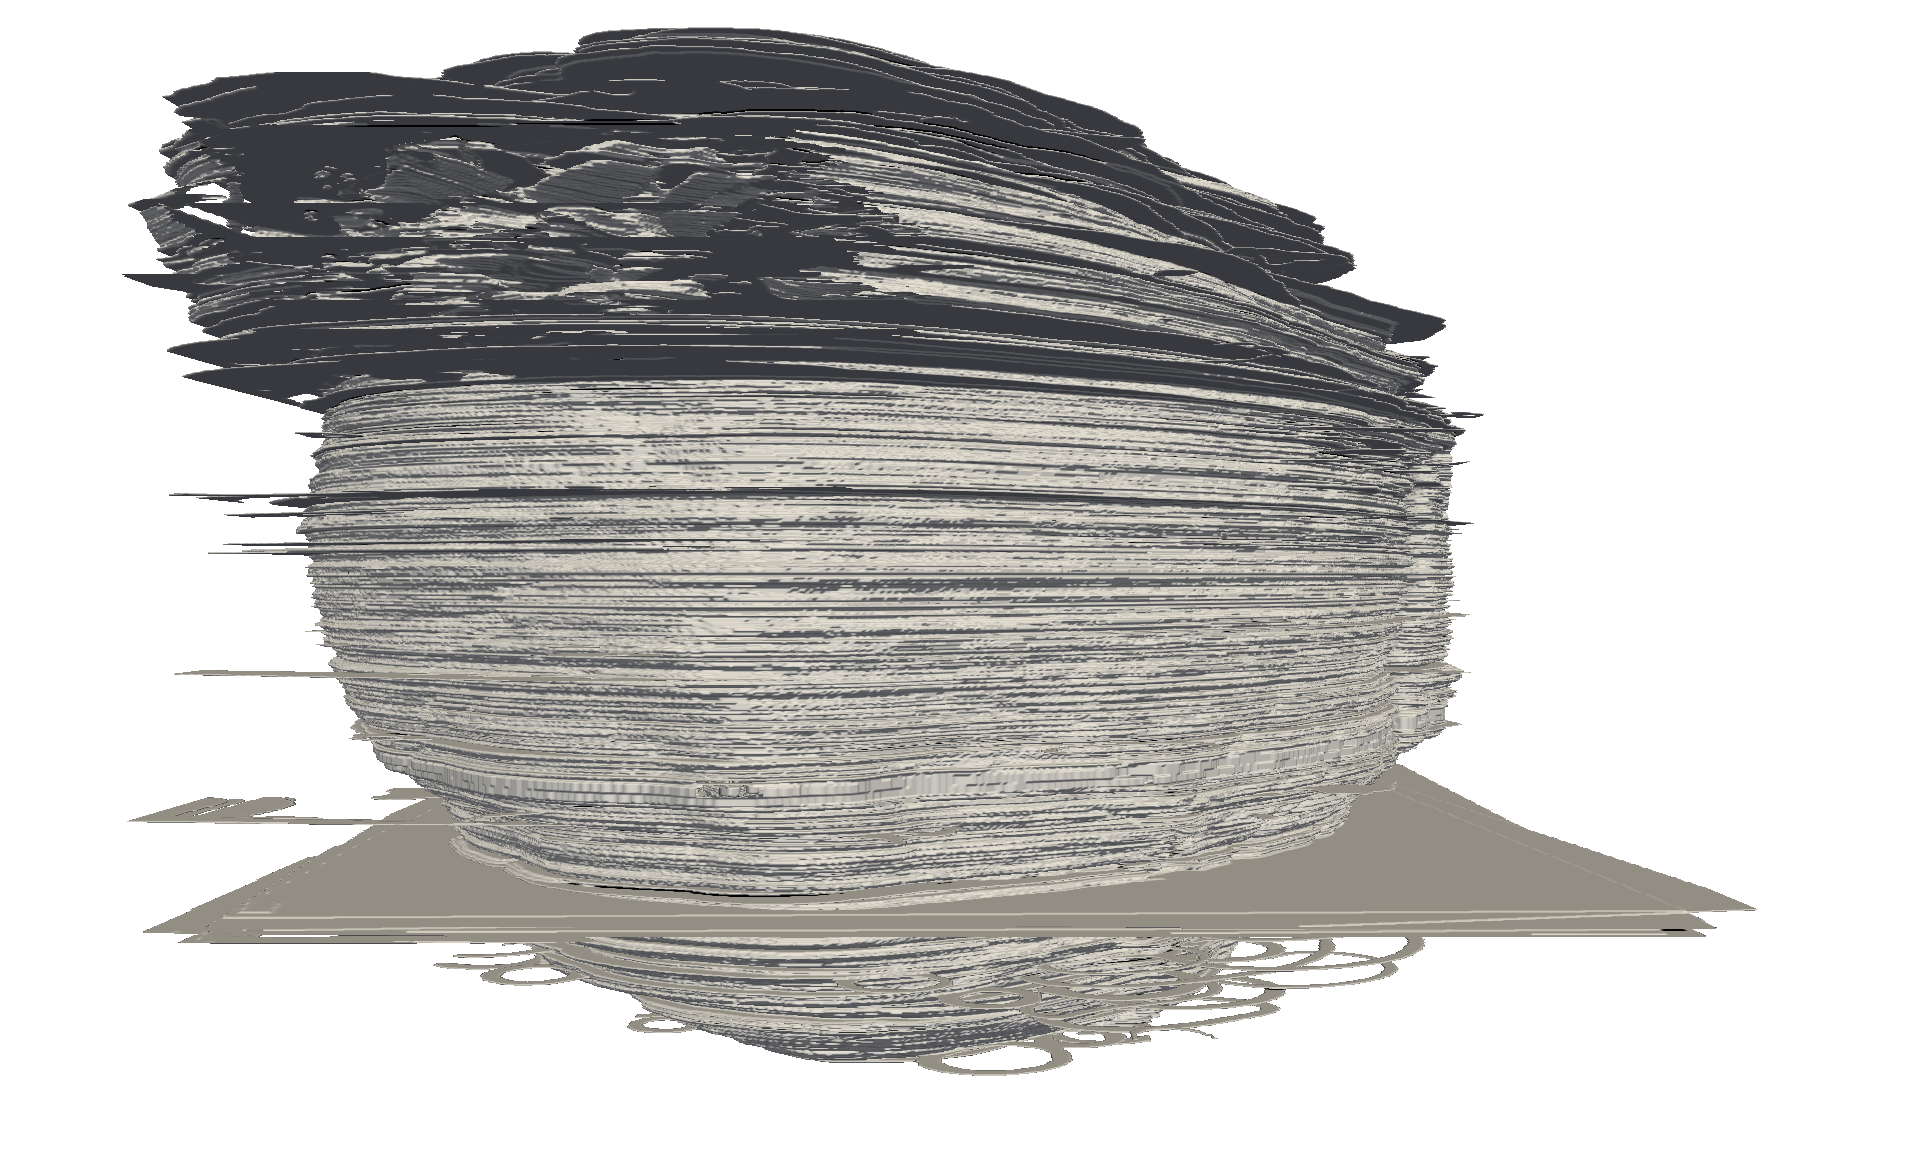
\includegraphics[width=0.9\textheight]{Ch6/Figs/Rat28/contours/whole_positive_y_diffused}
    \caption{Globally smoothed slice volume, viewed along the positive y direction.}
    \label{fig:whole_positive_y_diffused}
  \end{sidewaysfigure}
  
% chapter supplementary_images (end)
